\documentclass[9pt]{beamer}

% There are many different themes available for Beamer. A comprehensive
% list with examples is given here:
% http://deic.uab.es/~iblanes/beamer_gallery/index_by_theme.html

\usepackage[english]{babel}
\usepackage[sfdefault]{roboto}
\usepackage[T1]{fontenc}
\usepackage{array, booktabs}
\usepackage{multirow}
\usepackage{ulem}
\usepackage[flushleft]{threeparttable}
\usepackage[font=small,labelfont=bf]{caption}
\usepackage[utf8]{inputenc}
\usepackage{bookman}
\usepackage{mathtools}
\usepackage{kotex}
\usepackage{adjustbox} % for \adjincludegraphics
\usepackage{textcomp}
\usepackage{pdfpages}
\usepackage{listings}
\usepackage[framed,numbered,autolinebreaks,useliterate]{mcode}
\usepackage{color} %red, green, blue, yellow, cyan, magenta, black, white
\definecolor{mygreen}{RGB}{28,172,0} % color values Red, Green, Blue
\definecolor{mylilas}{RGB}{170,55,241}

\newcommand\ytl[2]{\parbox[b]{8em}{\hfill{\color{cyan}\bfseries\sffamily #1}~$\cdot$~}\makebox[0pt][c]{$\bullet$}\vrule\quad \parbox[c]{4.5cm}{\vspace{7pt}\color{red!40!black!80}\raggedright\sffamily #2.\\[7pt]}\\[-3pt]}

\usefonttheme{professionalfonts}

\usetheme{metropolis}

\setbeamertemplate{caption}[numbered]{}
\setbeamertemplate{navigation symbols}{}
\newcounter{frame}[frame]
\setbeamertemplate{footline}[frame number]

%\setbeameroption{show notes}

%\graphicspath{{./images/}}

\title{Artificial Neural-Network Based Hysteresis Identification}

\setbeamertemplate{footline}[text line]{%
  \parbox{\linewidth}{\vspace*{-8pt}\small SEEBUS 2022, Nagoya, Japan\hfill\hfill}}
%  
\setbeamertemplate{navigation symbols}{}

%\subtitle{Development of Monitoring Technique for Cultural Heritage Using Machine Learning-Based Kalman Filter}

\author{Sung-Yong Kim\inst{1}, Hong-Lae Jang\inst{2}, Cheol-Ho Lee\inst{3}}
% - Give the names in the same order as the appear in the paper.
% - Use the \inst{?} command only if the authors have different
%   affiliation.

\institute[CWNU] % (optional, but mostly needed)
{
	\inst{1}%
	Assistant Professor, School of Architecture, Changwon National University, Korea
	
	\inst{2}
	Assistant Professor, College of Mechatronics, Changwon National University, Korea
	
	\inst{3}
	Professor, Dept. of Architecture and Architectural Engineering, Seoul National University, Korea}
	
% - Use the \inst command only if there are several affiliations.
% - Keep it simple, no one is interested in your street address.

\date{December 14, 2022}
% - Either use conference name or its abbreviation.
% - Not really informative to the audience, more for people (including
%   yourself) who are reading the slides online

\subject{2022 SEEBUS}
% This is only inserted into the PDF information catalog. Can be left
% out. 

% If you have a file called "university-logo-filename.xxx", where xxx
% is a graphic format that can be processed by latex or pdflatex,
% resp., then you can add a logo as follows:

%\pgfdeclareimage[height=0.5cm]{university-logo}{cwnu_logo}
%\logo{\pgfuseimage{cwnu_logo}}



% Let's get started
\begin{document}

\lstset{language=Matlab,%
    basicstyle=\color{red},
    breaklines=true,%
    morekeywords={matlab2tikz},
    keywordstyle=\color{blue},%
    morekeywords=[2]{1}, keywordstyle=[2]{\color{black}},
    identifierstyle=\color{black},%
    stringstyle=\color{mylilas},
    commentstyle=\color{mygreen},%
    showstringspaces=false,%without this there will be a symbol in the places where there is a space
    numbers=left,%
    numberstyle={\tiny \color{black}},% size of the numbers
    numbersep=9pt, % this defines how far the numbers are from the text
    emph=[1]{for,end,break},emphstyle=[1]\color{red}, %some words to emphasise
    %emph=[2]{word1,word2}, emphstyle=[2]{style},    
}


\begin{frame}
	\titlepage
\end{frame}
\begingroup
\setbeamertemplate{footline}[text line]{%
  \parbox{\linewidth}{\vspace*{-8pt}\small \hfill\hfill\insertpagenumber /28}}

\begin{frame}{Outline}
    \tableofcontents
\end{frame}

\section{Introduction}

\begin{frame}{Motivation of this study}
Question: Why do we conduct component-level tests?

My answer: 
\begin{itemize}
	\item To build a theoretical model based on the test results
	\item To evaluate the seismic behavior and performance of the whole structural system
\end{itemize}

Technical issues:
\begin{itemize}
	\item How to build a theoretical model based on the test results?
	\item How to evaluate the global behavior and performance of the system?
\end{itemize}
\end{frame}

\begin{frame}{Solution of Ordinary Differential Equations}
\begin{columns}
\begin{column}{0.5\textwidth}
\begin{figure}
	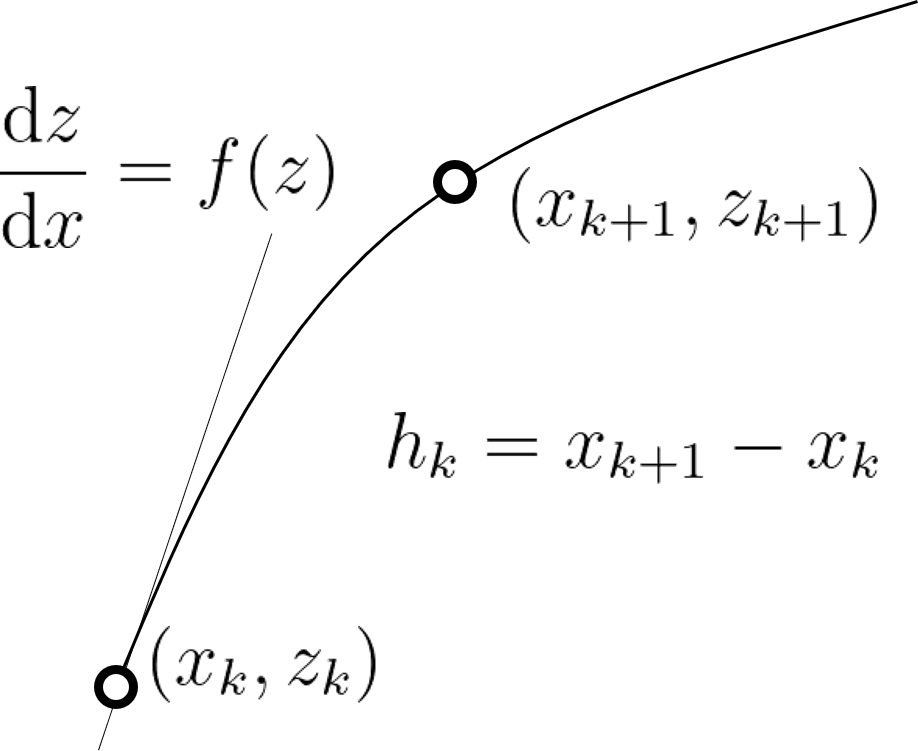
\includegraphics[height=.4\textheight]{ODEfigure}
	\caption{Schematic diagram of an ODE and its solution: $(x_k,z_k)$ is the current state, $f(\cdot)$ is the derivative, and $h_k$ is the step size.}
\end{figure}
\end{column}
\begin{column}{0.5\textwidth}  %%<--- here
\begin{itemize}
	\item Euler's method: 
	\[z_{k+1} = z_k + h_k f(z_k)\]
	\item Runge-Kutta's method (RK4):
	\[z_{k+1} = z_k + \frac{h_k}{6}(k_1 + 2k_2 + 3k_2 + k_4)\]
	\noindent where
	\[k_1 = f(z_k)\]
	\[k_2 = f(z_k + h_k k_1/2)\]
	\[k_3 = f(z_k + h_k k_2/2)\]
	\[k_4 = f(z_k + h_k k_3)\]
\end{itemize}
\end{column}
\end{columns}
\vspace{.5cm}
When the form of the differential equation is known, it is well known how to calculate the value of the next step from the current step (e.g., Euler's method, and Runge-Kutta's method).
\end{frame}
\note{There are many technical methods to solve the given ODE. At the point ($x_k, z_k$), the approximation $z_{k+1}$ can be estimated with the help of the given function $f$. This method is called Euler’s method. Here is another way of solving a given ODE: RK4. Starting with the simple Euler approximation, four adequate approximate values are determined, then the values are weighted appropriately used for the approximation.}

\begin{frame}{Determination of Best Fitting ODE Model}
\begin{figure}
	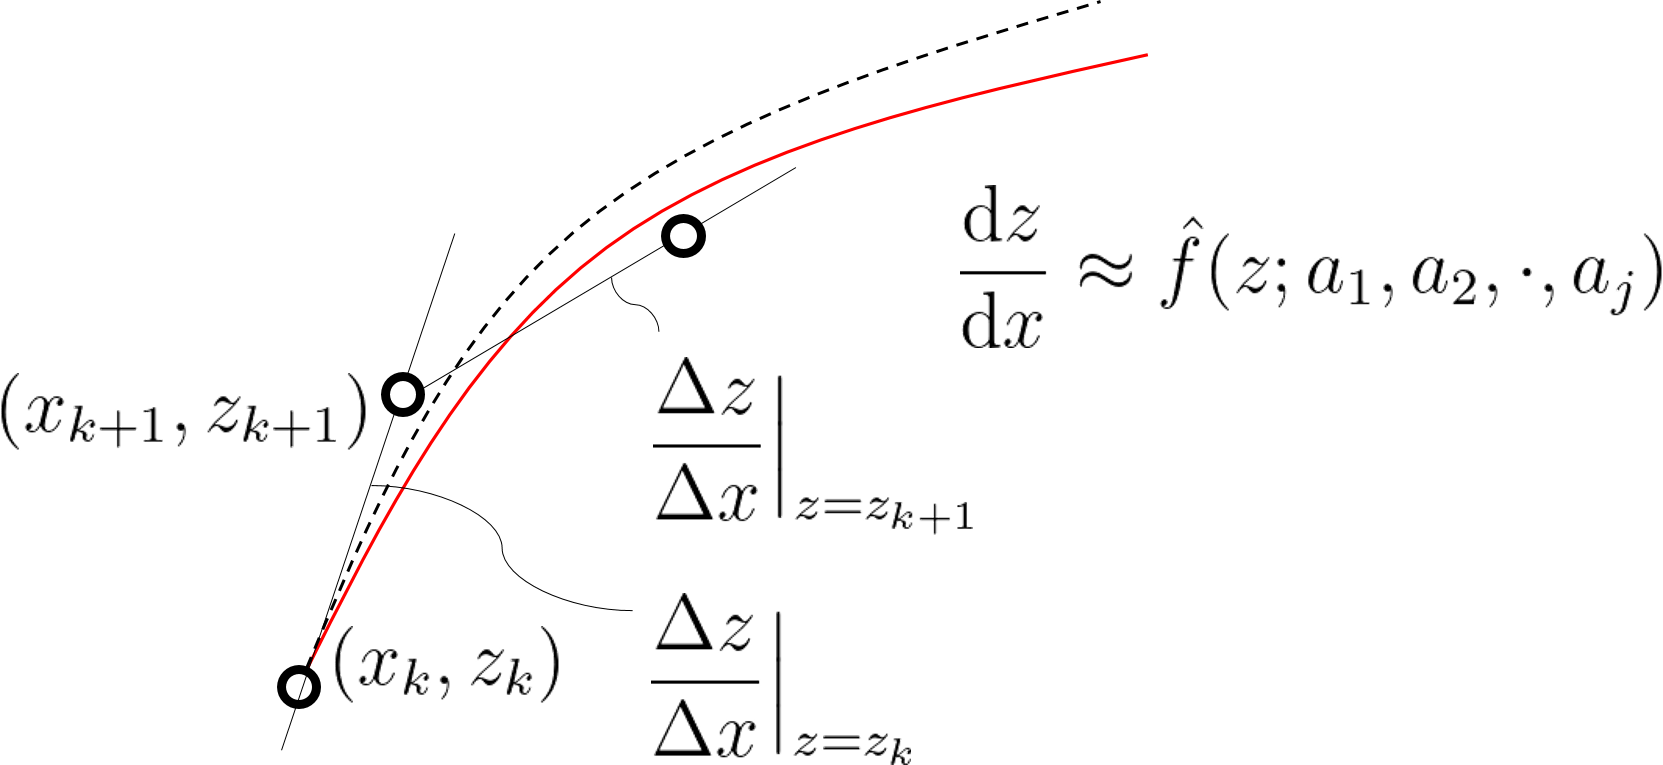
\includegraphics[height=.4\textheight]{ODEfigure2}
	\caption{Given data and determination of best ODE model: $\hat f(\cdot)$ represents the estimated ODE model, and $a_1,\cdots,a_j$ are best-fitting parameters.}
\end{figure}
Given the data, we choose a model that is thought to be appropriate and determine the model's best-fitting parameters.
\end{frame}

\begin{frame}{Determination of Best Fitting Hysteresis Model}
\begin{figure}
	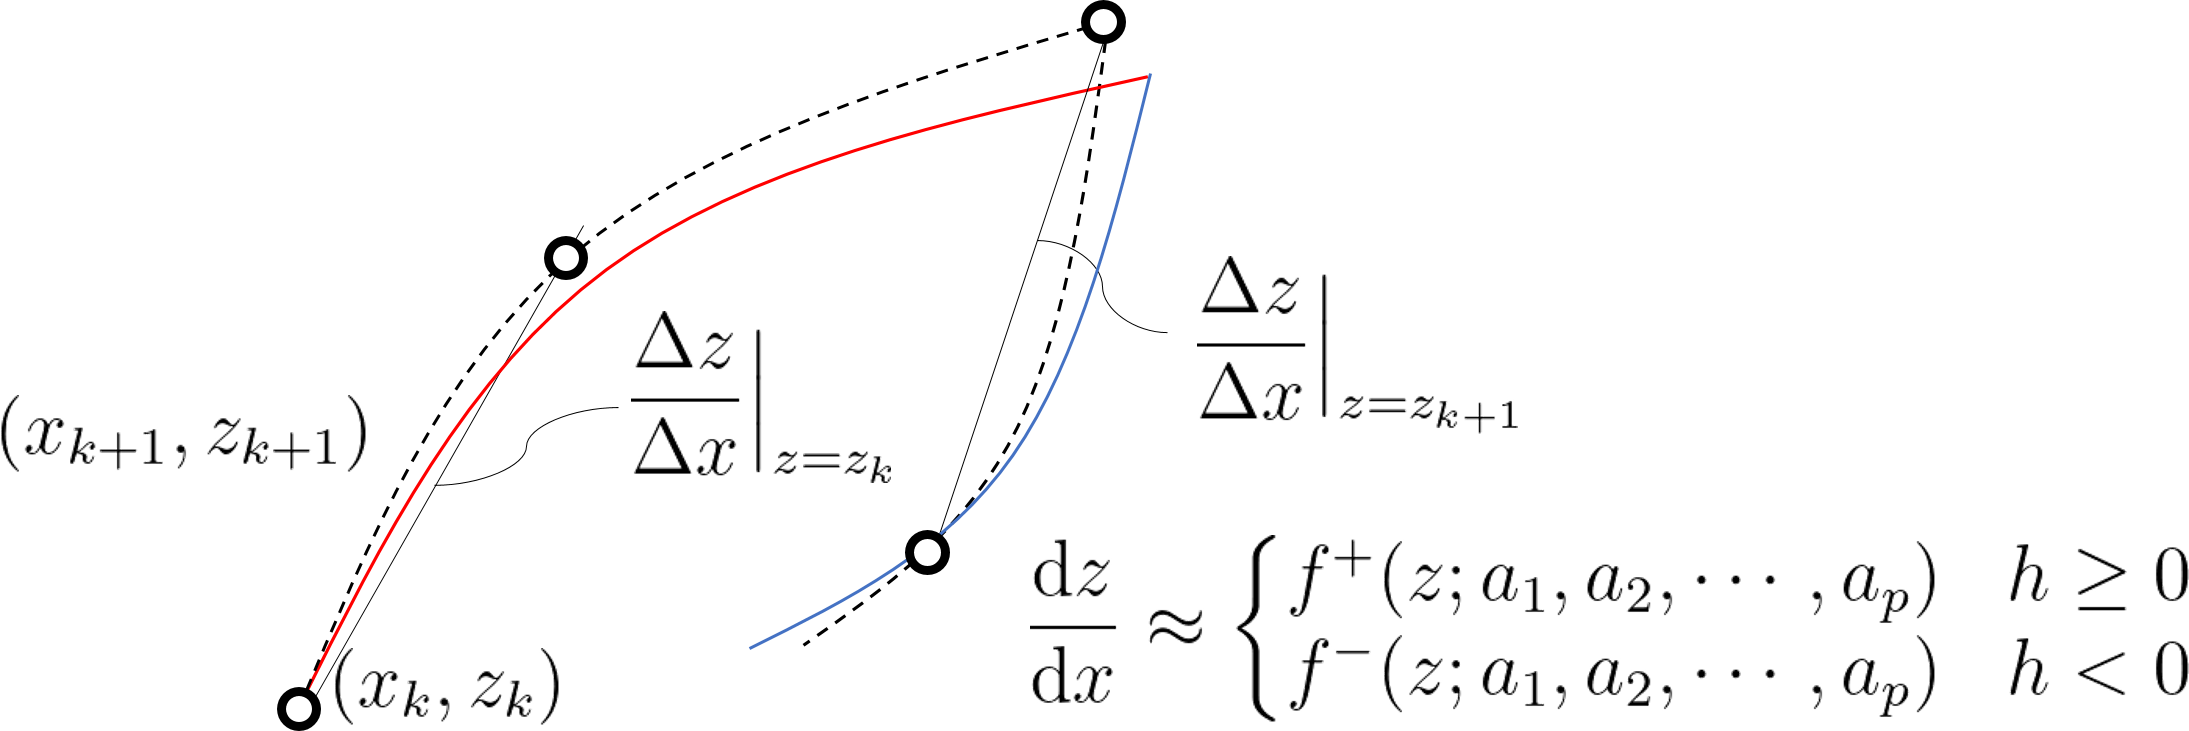
\includegraphics[height=.4\textheight]{ODEfigure3}
	\caption{Schematic diagram of a hysteresis loop: loading stage (red) and unloading stage (blue); $f^+(\cdot)$ and $f^-(\cdot)$ are functions for loading and unloading stages, respectively.}
\end{figure}
Hysteresis models are not significantly different from ODEs. To describe the hysteretic behavior, it is necessary to define the different functions for both loading and unloading stages separately.
\end{frame}

\begin{frame}{Example: Bouc-Wen Model}
\begin{columns}
\begin{column}{0.4\textwidth}
\begin{figure}
	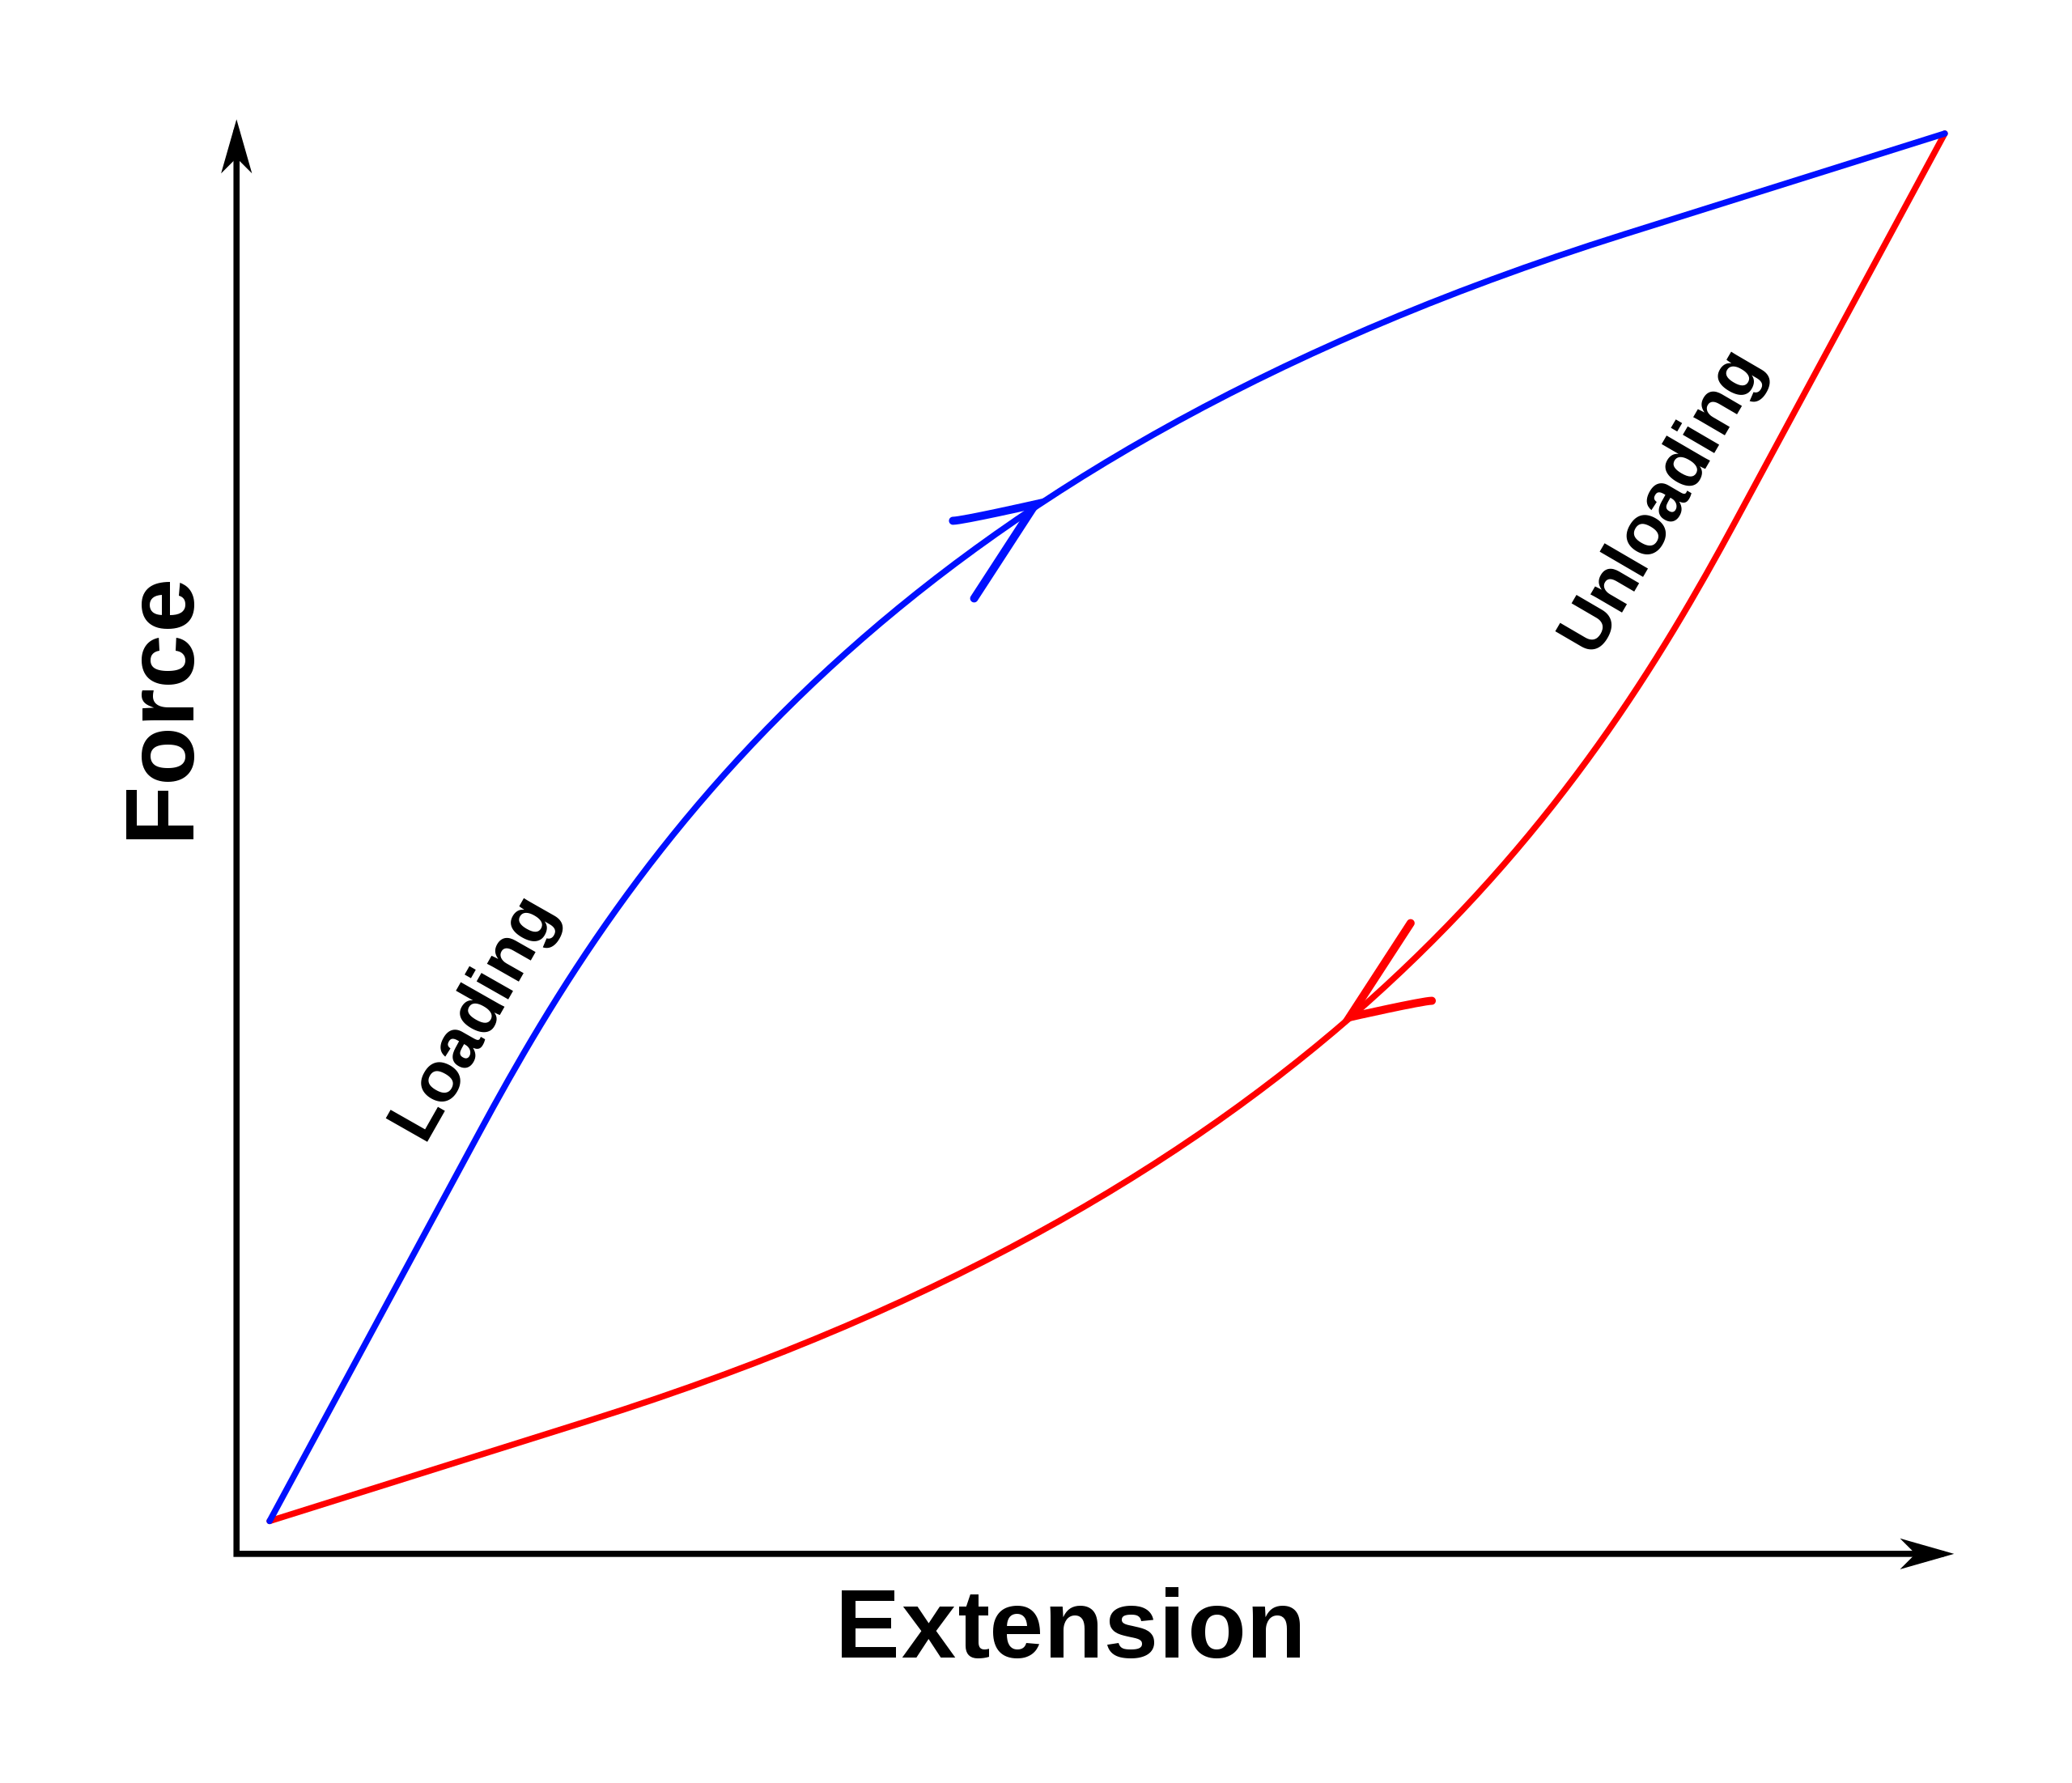
\includegraphics[height=.55\textheight]{example01}
	\caption{Hysteresis model}
\end{figure}
\end{column}
\begin{column}{0.6\textwidth}  %%<--- here
\begin{itemize}
	\item Bouc-Wen Model
	\[\frac{\mathrm dz}{\mathrm dx}=
A-\vert z\vert^n[\gamma-\beta\mathrm{sgn}(z\mathrm dx)]\]
\noindent \[a_1=A,a_2=\beta,a_3=\gamma,a_4=n,\]
	\[f^+(z;a_1,a_2,a_3,a_4)= a_1 - \vert z\vert^{a_4}(a_3 - a_2)\]
	\[f^-(z;a_1,a_2,a_3,a_4)= a_1 - \vert z\vert^{a_4}(a_3 + a_2)\]	
\end{itemize}
\end{column}
\end{columns}
\begin{itemize}
	\item Given the data, we can choose a model that is thought to be appropriate and can determine the model's best-fitting parameters.
	\item Once we bulid a model, we again have to solve the differential equation. 
	\item Is there any model which is easy to build, and is easy to solve?
\end{itemize}

\end{frame}

\begin{frame}{Neural Networks and Universal Approximation Theorem}
Consider a nonlinear system described by the following ODE:

\begin{equation}
 \frac{\mathrm dz}{\mathrm dx} = f(z)
\end{equation}

\noindent with initial value $z(0) = z_o$. 

The following theorem shows the existence of a neural network that meets the required property. 

\begin{theorem}[Universal Approximation Theory of Neural Network]
Given any solution trajectory $z(x;z_o)$ of the system described in Eq.(1) with $z_o\in D$, and a function is continuous and satisfies the Lipschitz condition, for any $\varepsilon > 0$, \textcolor{red}{there exists a neural network $N_f(\cdot)$ such that the trajectory corresponding to the system $y'=N_f(y)$, $y(0)=z_o$ satisfies $\Vert y(x;z_o) - z(x;z_o)\Vert < \varepsilon$, for any $z_o\in D$.} 
\end{theorem}

%However, it dose not indicate how such a network can be obtained. VERY CAREFUL IN APPLYING SUCH A MODEL
\end{frame}

\section{Proposed Model}

\begin{frame}{Proposed Model}

\hrulefill
\[z_{k+1} = N(x_k,h_k,z_k)\]
\noindent where $x_k$ is the displacement at the $k$-th step, $h_k=x_{k+1} - x_k$ is the step size, and $z_k$ is the force at the $k$-th step.

\hrulefill

Main objective of this study is to construct a model, which is
\begin{itemize}
	\item easy to build, and
	\item easy to solve.   
\end{itemize}

\[z_{k+1} = z_k + h_k f(z_k) \rightarrow z_{k+1} = z_k + h_k N_f(z_k) \rightarrow z_{k+1} = z_k + \hat N_f(h_k,z_k)\]
In order to satisfy the above objectives, we 
\begin{itemize}
	\item build a neural net-based model, and
	\item constructed a training set so that the solution does not depend on the time step.
\end{itemize}
\end{frame}

\begin{frame}{Rearrangement of Dataset}
\begin{columns}
\begin{column}{0.4\textwidth}
\begin{figure}
	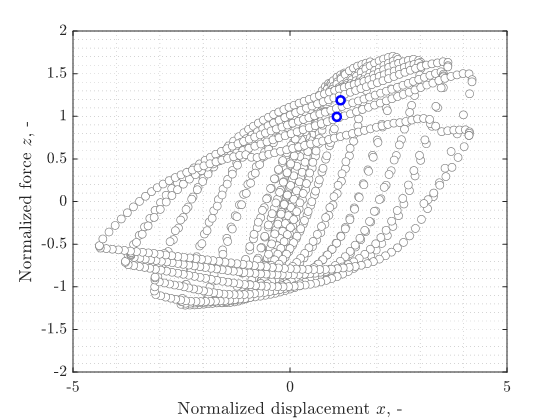
\includegraphics[height=.45\textheight]{dataSelection01}
	\caption{Hysteresis loop and data selection}
\end{figure}
\end{column}
\begin{column}{0.58\textwidth}  %%<--- here
\begin{itemize}
	\item 0. Original test results
	\begin{table}
%	\centering
\small
\begin{tabular}{@{}cc@{}}
\toprule
Input & Output \\ 
$x_k$ & $z_k$ \\ \midrule
0.00 & 0.00 \\ 
0.10 & 0.20 \\ 
0.20 & 0.40 \\
\vdots & \vdots \\ 
\bottomrule 
\end{tabular} 	
	\end{table}
\item 1. Rearrange the dataset: Input ($x_k, h_k$ and $z_k$) and output ($z_{k+1}$)
	\begin{table}
%	\centering
\small
\begin{tabular}{@{}cccc@{}}
\toprule
\multicolumn{3}{c}{Input} & Output \\ 
$x_k$ & $h_k=x_{k+1}-x_k$ & $z_k$ & $z_{k+1}$\\ \midrule
0.00 & 0.10 & 0.10 & 0.00 \\ 
0.10 & 0.10 & 0.20 & 0.10 \\ 
\vdots & \vdots & \vdots & \vdots \\ 
\bottomrule 
\end{tabular} 	
	\end{table}
\end{itemize}
\end{column}
\end{columns}
\end{frame}

\begin{frame}{Error Due to Biased Training Set Selection}
\begin{figure}
	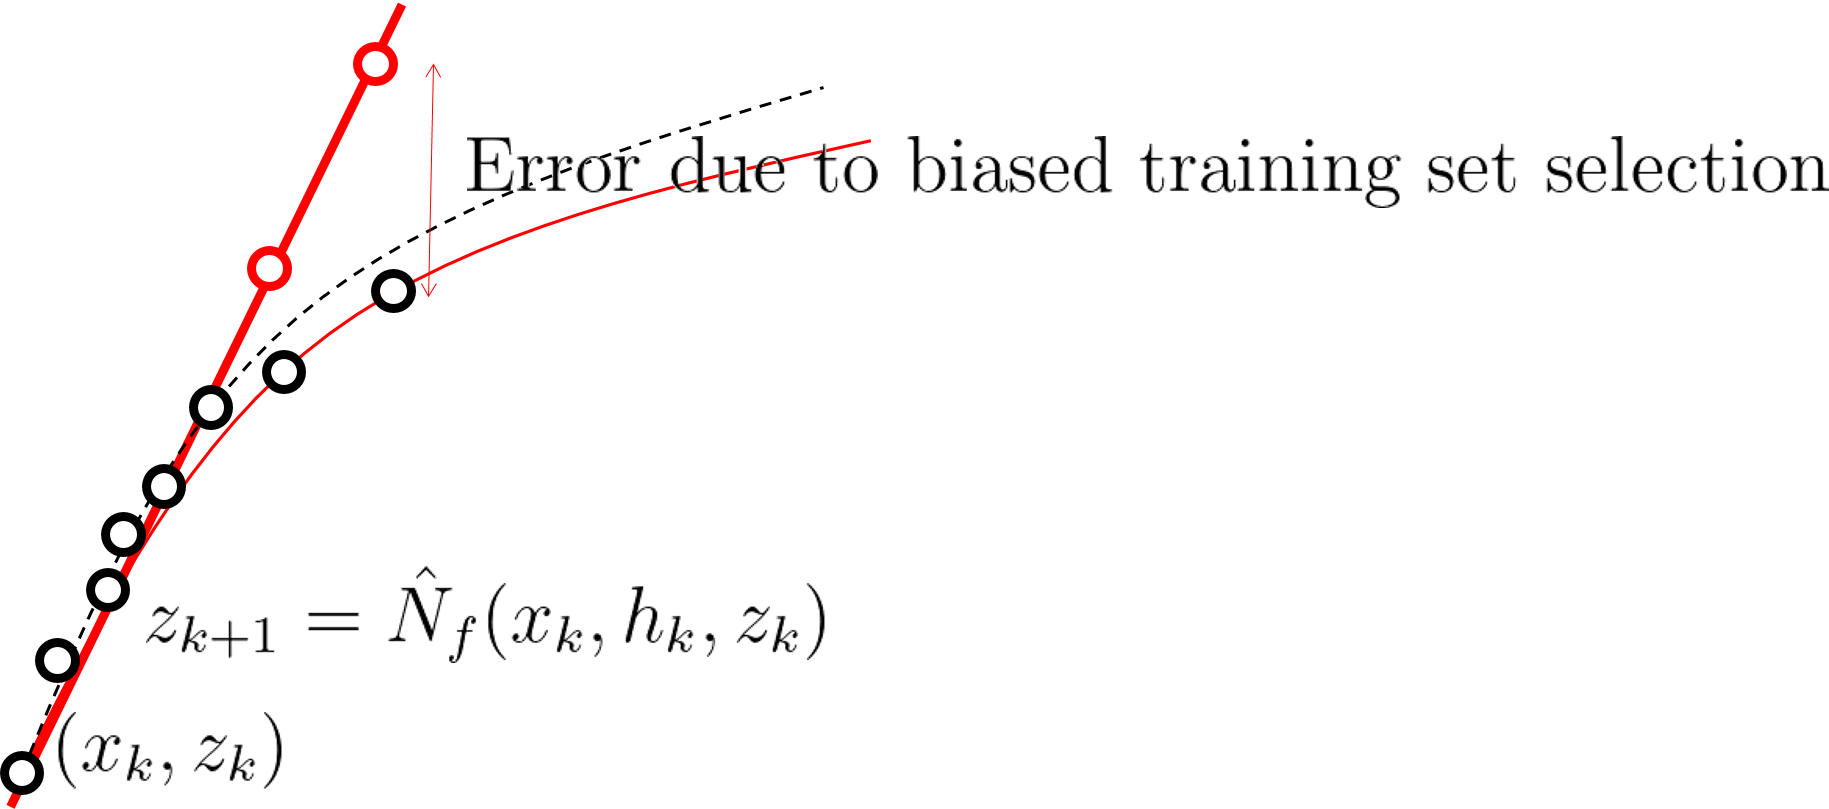
\includegraphics[height=.4\textheight]{scheme02}
	\caption{Test (left) and error (right)}
\end{figure}

\vspace{.5cm}
If a neural network is trained with biased data (or only with small-step data), the results can be also biased. $\rightarrow$ May give us stiffer prediction. $\rightarrow$ Data should be augmented such that various sizes of step size are included. 
\end{frame}

\begin{frame}{Augmentation of Dataset (Key feature of this study)}
\begin{columns}
\begin{column}{0.4\textwidth}
\begin{figure}
	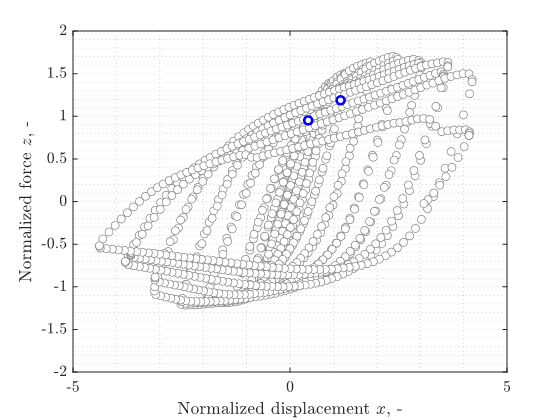
\includegraphics[height=.45\textheight]{dataSelection02}
	\caption{Augmentation of input data}
\end{figure}
\end{column}
\begin{column}{0.58\textwidth}  %%<--- here
\begin{itemize}
\item[3.] Rearrange the dataset
	\begin{table}
%	\centering
\small
\begin{tabular}{@{}cccc@{}}
\toprule
\multicolumn{3}{c}{Input} & Output \\ 
$x_k$ & $h_k=x_{k+1}-x_k$ & $z_k$ & $z_{k+1}$\\ \midrule
0.00 & 0.10 & 0.10 & 0.00 \\ 
0.10 & 0.10 & 0.20 & 0.10 \\ 
\vdots & \vdots & \vdots & \vdots \\ 
\bottomrule 
\end{tabular} 	
	\end{table}
\item[4.] Augment the dataset
	\begin{table}
%	\centering
\small
\begin{tabular}{@{}cccc@{}}
\toprule
\multicolumn{3}{c}{Input} & Output \\ 
$x_k$ & $h_k=x_{k+1}-x_k$ & $z_k$ & $z_{k+1}$\\ \midrule
0.00 & 0.10 & 0.10 & 0.00 \\ 
0.10 & 0.20 & 0.10 & 0.20 \\ 
\vdots & \vdots & \vdots & \vdots \\ 
\bottomrule 
\end{tabular} 	
	\end{table}
\end{itemize}
\end{column}
\end{columns}
\end{frame}

\begin{frame}{Construction of Neural Network}
\begin{figure}
	\includegraphics[height=.4\textheight]{NeuralNet}
	\caption{Test (left) and error (right)}
\end{figure}

\vspace{.5cm}
\begin{itemize}
	\item Software: MATLAB\texttrademark R2022a for academic use, Deep learning toolbox
	\item Hardware: Intel(R) Core(TM) i7-8550U CPU @ 1.80GHz (RAM 16.0GB)
	\item Total training time: 10--15 min
\end{itemize}
\end{frame}

\begin{frame}[fragile]
\scriptsize

	\begin{lstlisting}
[trainInd,valInd] = dividerand(numValidation,0.8,0.2);

xTrain = xPool(:, trainInd);
yTrain = yPool(:, trainInd);

xValid = xPool(:, valInd);
yValid = yPool(:, valInd);

%% Neural Network
layers = [ ...
    featureInputLayer(3, "Input", "myFeatureInputLayer", 'Normalization','rescale-symmetric')
    fullyConnectedLayer(5, "Hidden1", "myFullyConnectedLayer1")
    tanhLayer("Name", "myTanhLayer")
     fullyConnectedLayer(5, "Hidden2", "myFullyConnectedLayer2")
    tanhLayer("Name", "myTanhLayer2")   
    fullyConnectedLayer(1, "Output", "myFullyConnectedLayer3")
    regressionLayer("Name", "myRegressionLayer")
];

opts = trainingOptions('adam', ...
    'MaxEpochs',1500, ...
    'InitialLearnRate',0.01,...
    'Shuffle','every-epoch', ...
    'Plots','training-progress', ...
    'MiniBatchSize',128, ...
    'Verbose',false, ...
    'ValidationData', {xValid', yValid'});
	\end{lstlisting}
\end{frame}
%


\section{Validation of Proposed Model}
\begin{frame}{Example 1: Bouc-Wen Model}
\begin{figure}
	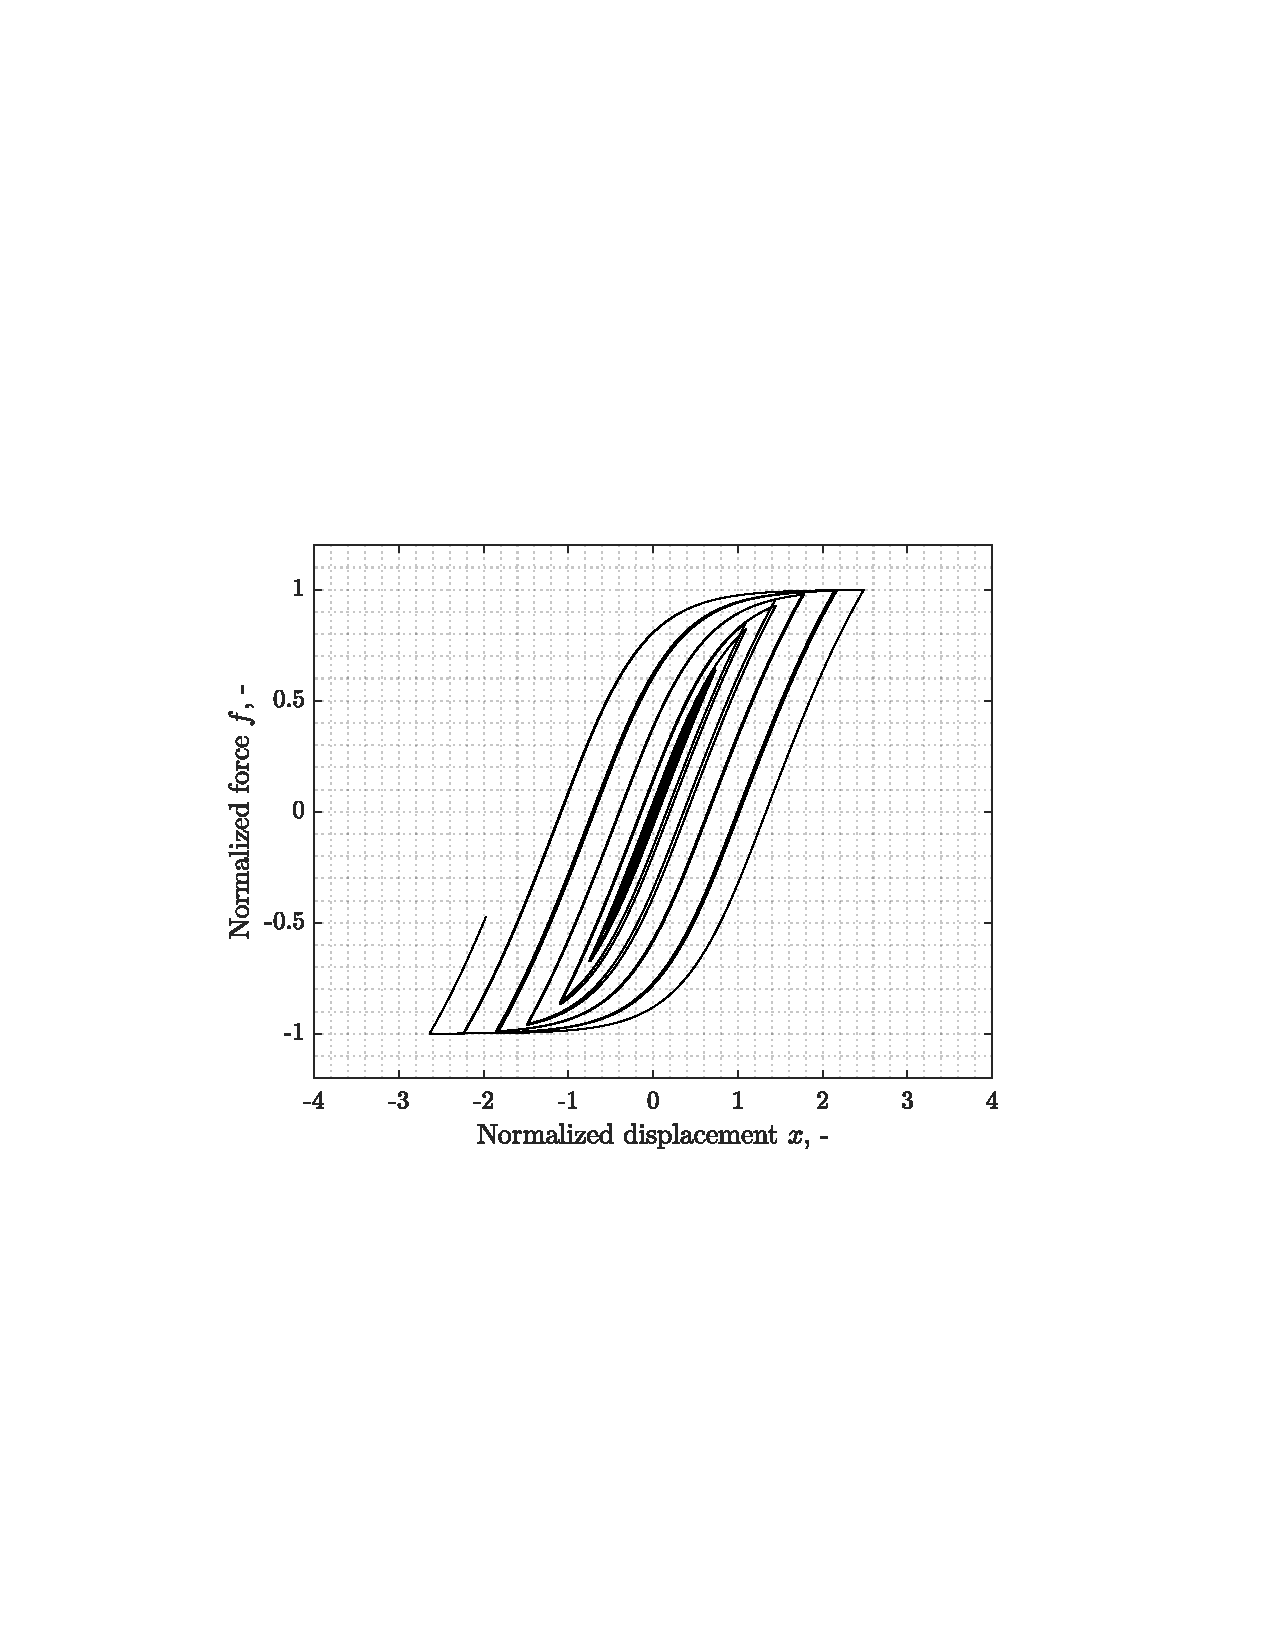
\includegraphics[height=.8\textheight]{neuralNetHysteresis01}
	\caption{Test set: Bouc-Wen model (simulated)}
\end{figure}
\end{frame}

\begin{frame}{Example 1: Training History}
\begin{figure}
	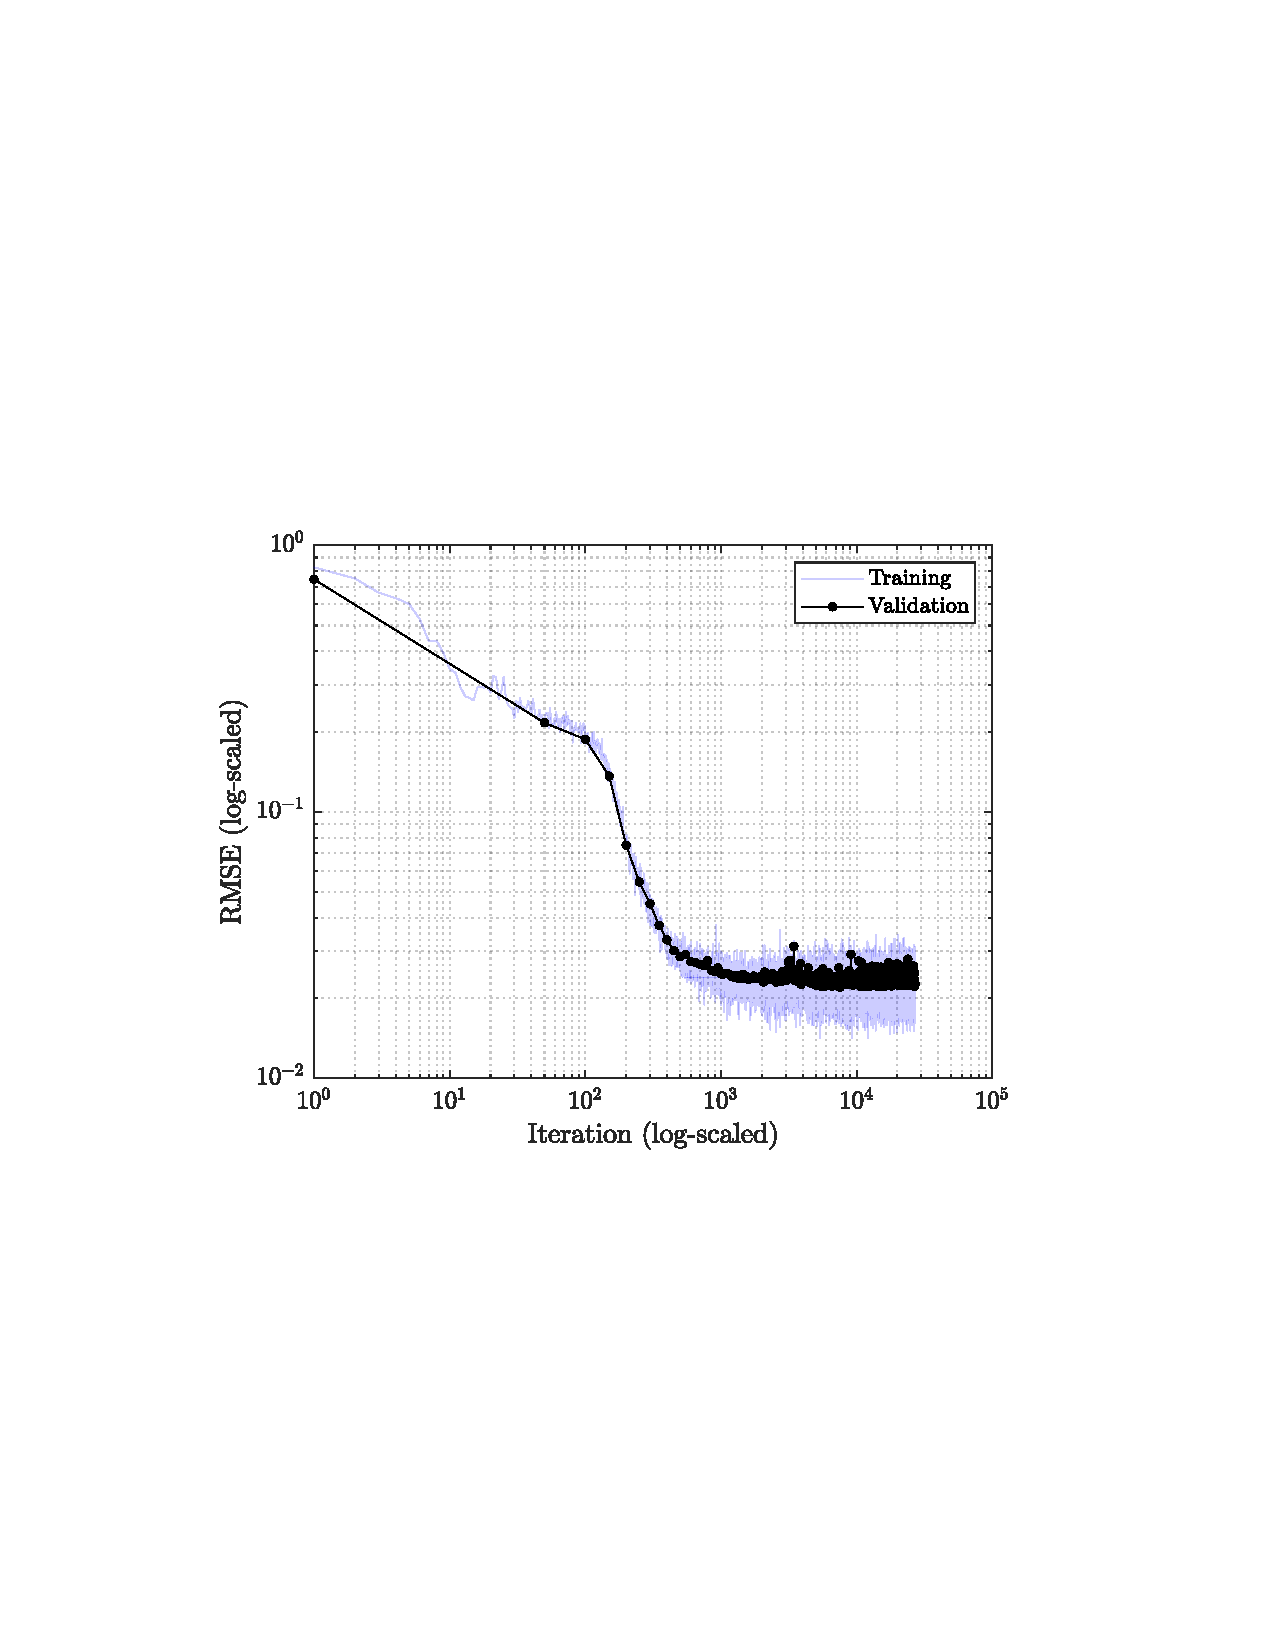
\includegraphics[height=.8\textheight]{neuralNetHysteresis01RMSE}
	\caption{Training history for Example 1}
\end{figure}
\end{frame}

\begin{frame}{Example 1: Validation Results}
\begin{figure}
	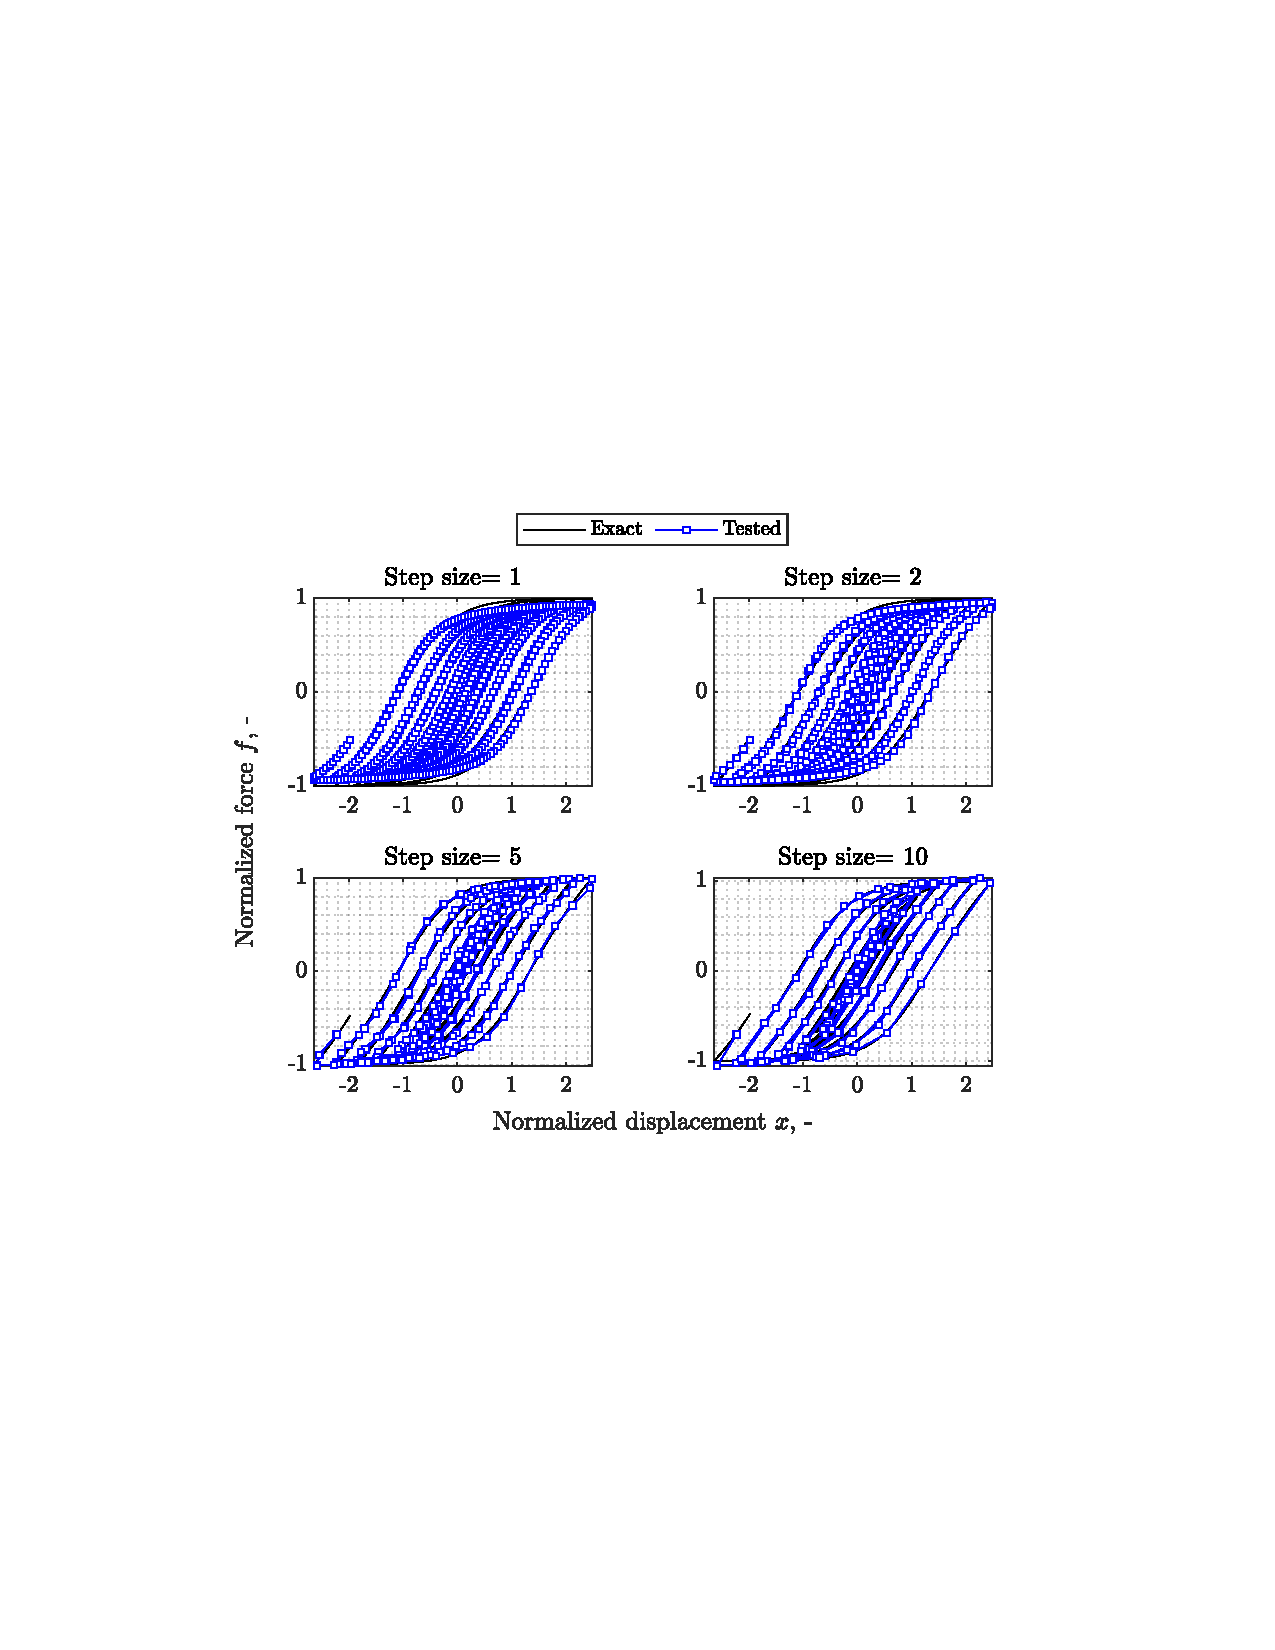
\includegraphics[height=.8\textheight]{neuralNetHysteresis01Test}
	\caption{Validation results}
\end{figure}
\end{frame}

\begin{frame}{Example 2: Bouc-Wen Model with Pinching Degradation}
\begin{figure}
	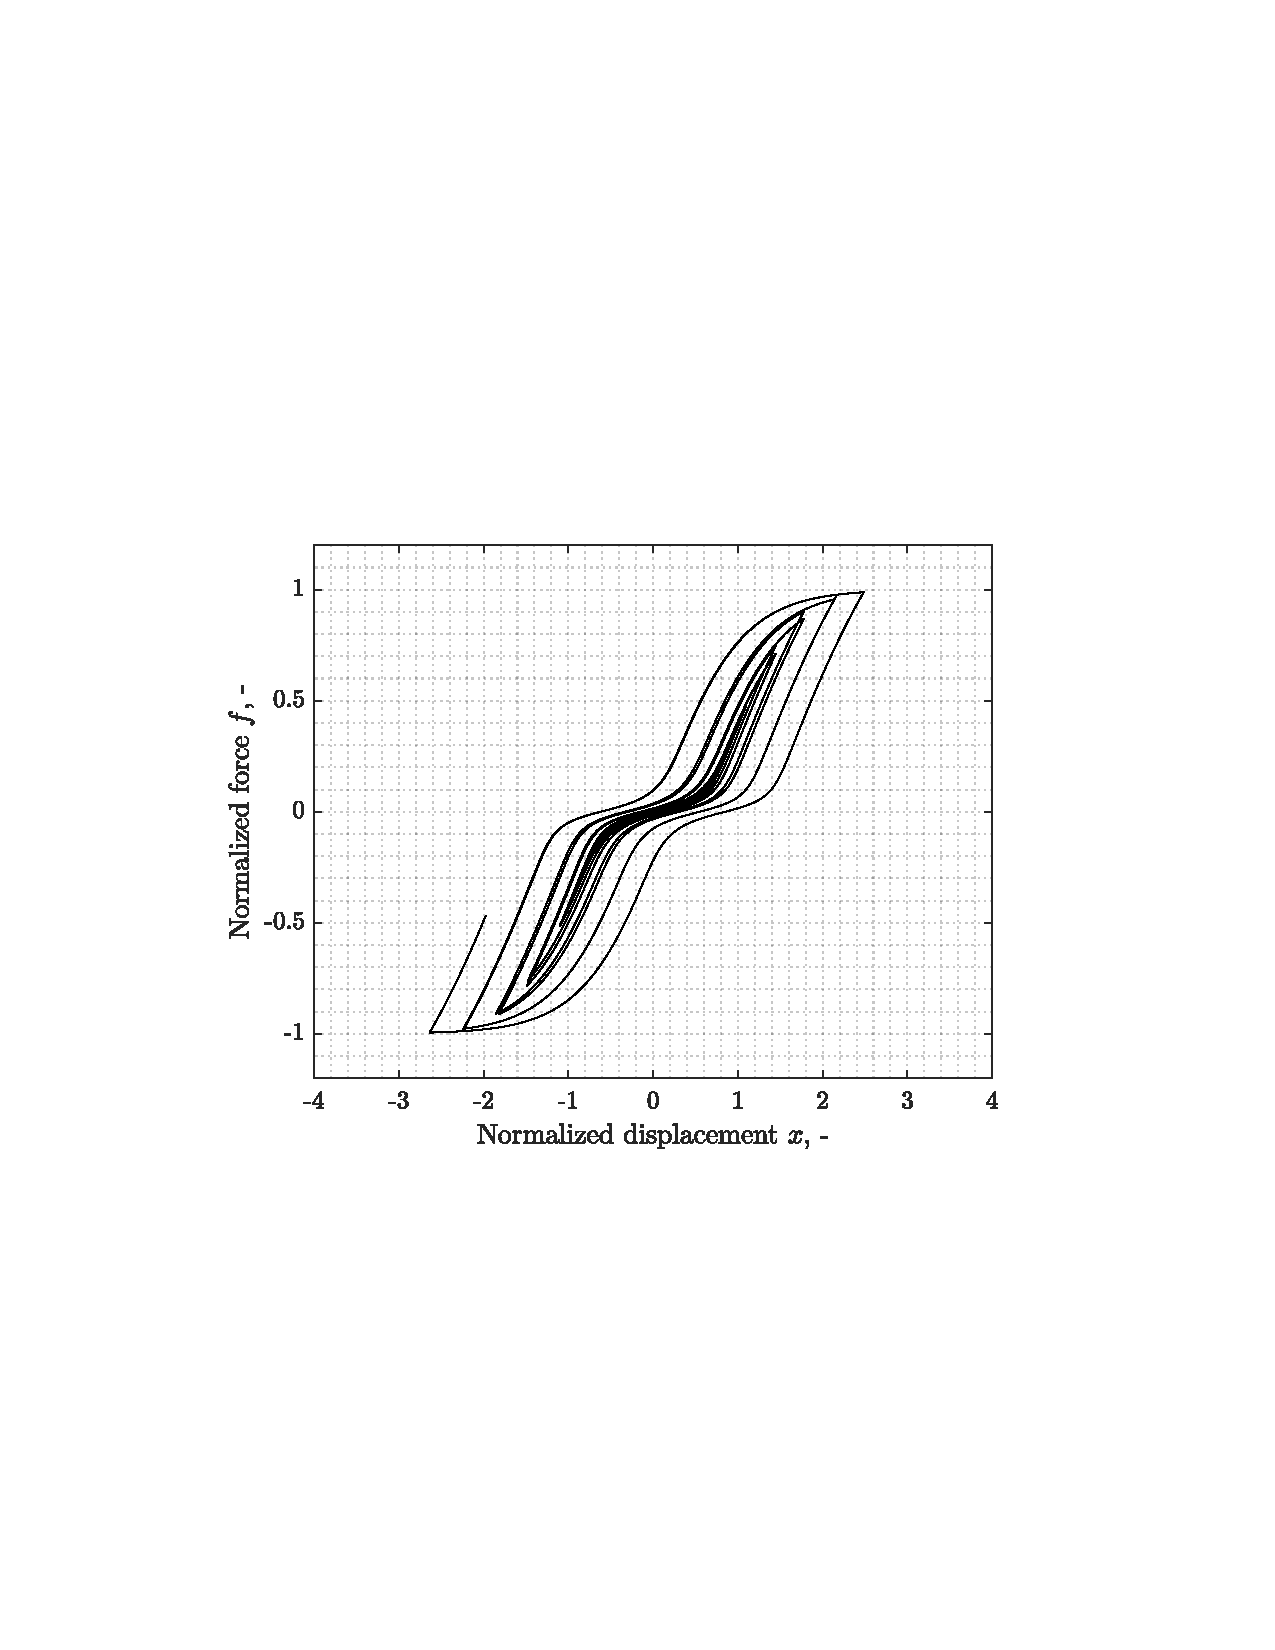
\includegraphics[height=.8\textheight]{neuralNetHysteresis02}
	\caption{Test set: Bouc-Wen model with pinching degradation (simulated)}
\end{figure}
\end{frame}

\begin{frame}{Example 2: Training History}
\begin{figure}
	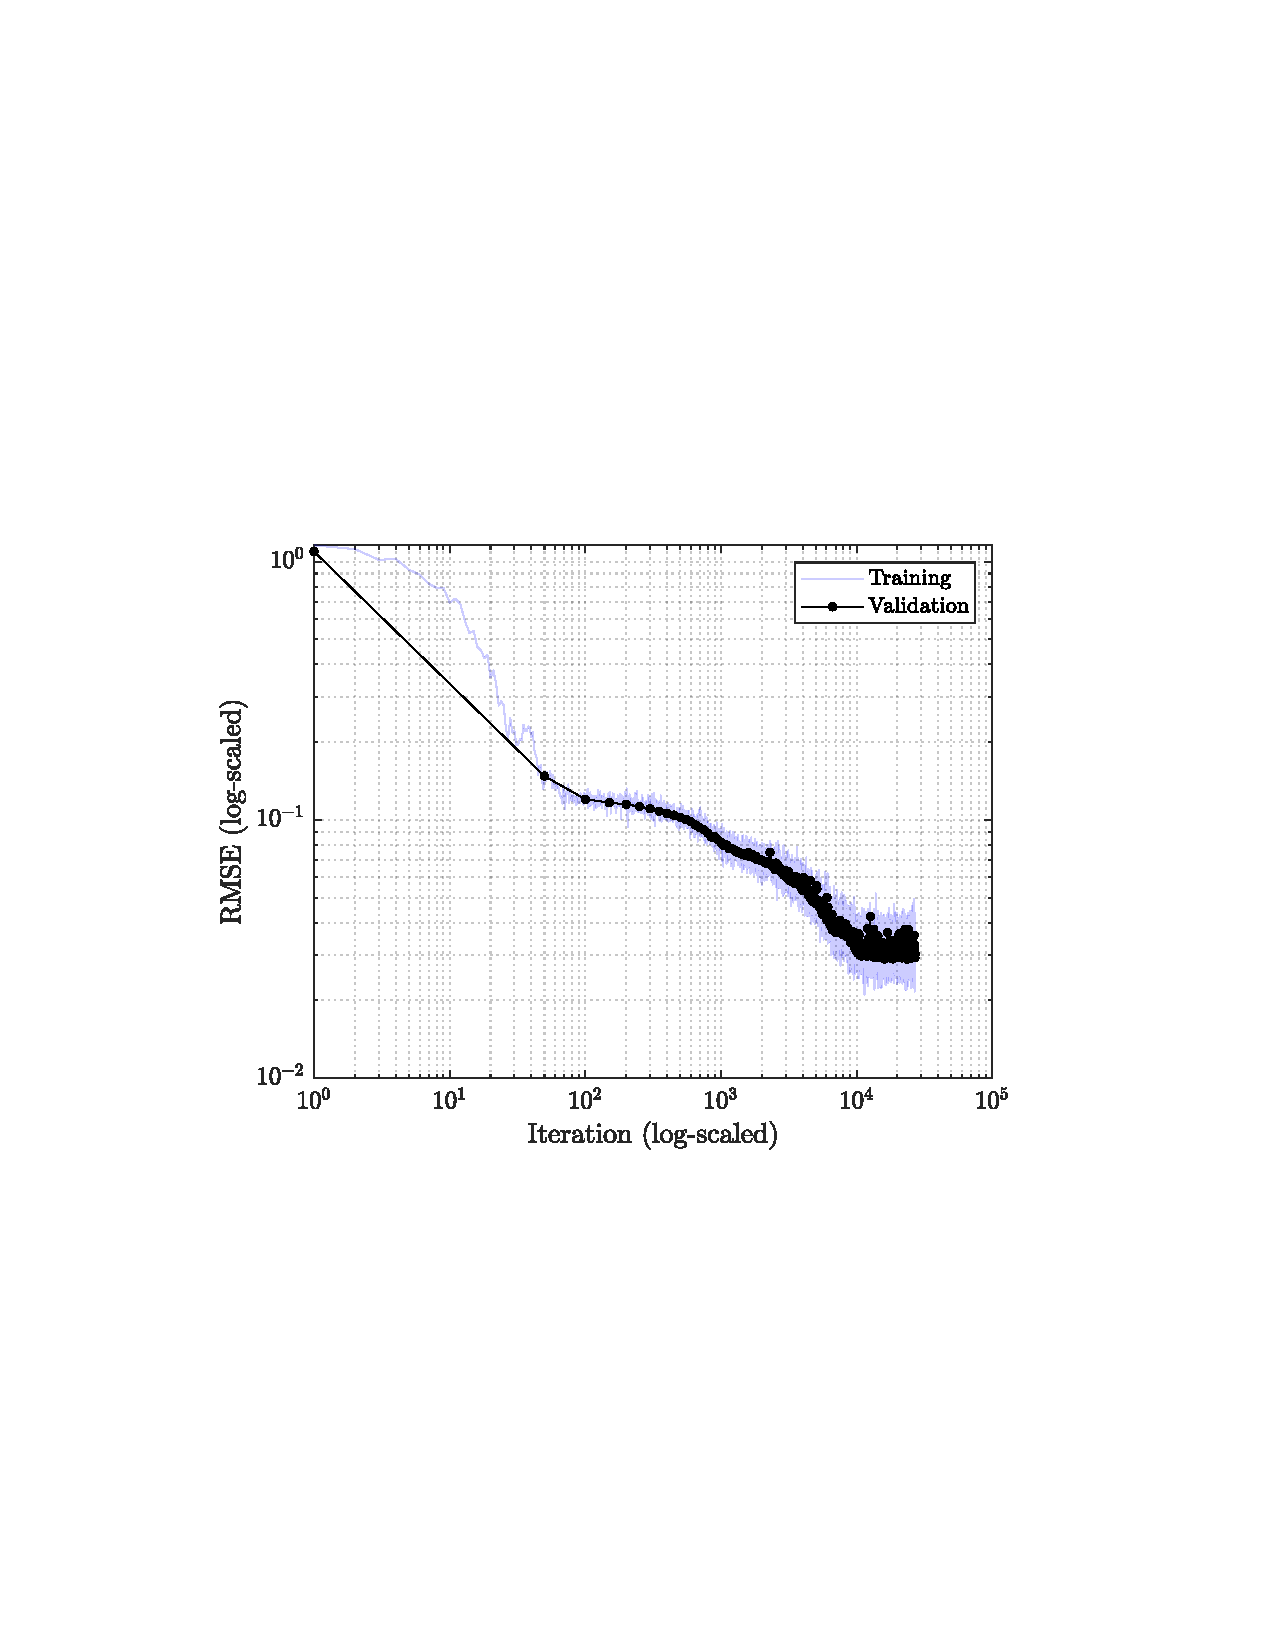
\includegraphics[height=.8\textheight]{neuralNetHysteresis02RMSE}
	\caption{Training history for Example 2}
\end{figure}
\end{frame}

\begin{frame}{Example 2: Validation Results}
\begin{figure}
	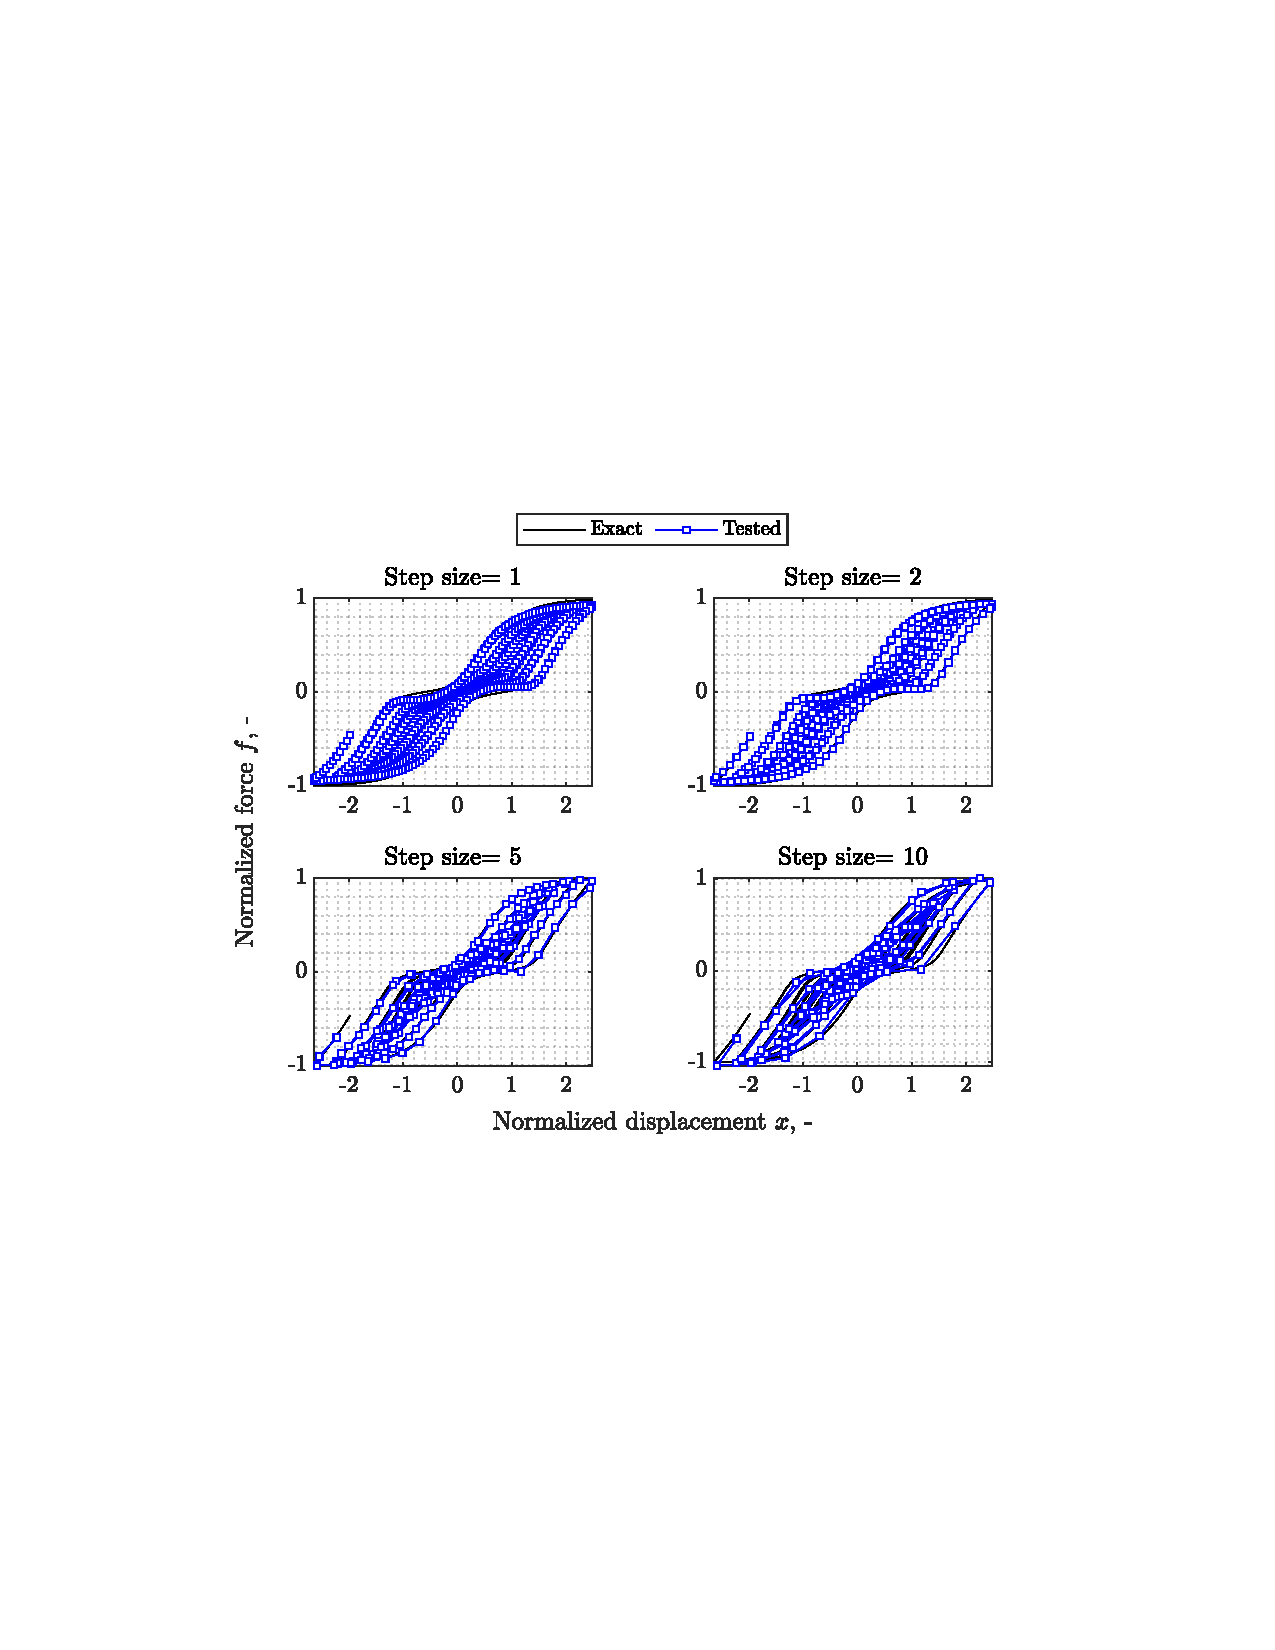
\includegraphics[height=.8\textheight]{neuralNetHysteresis02Test}
	\caption{Validation results}
\end{figure}
\end{frame}

\begin{frame}{Example 3: Training History}
\begin{figure}
	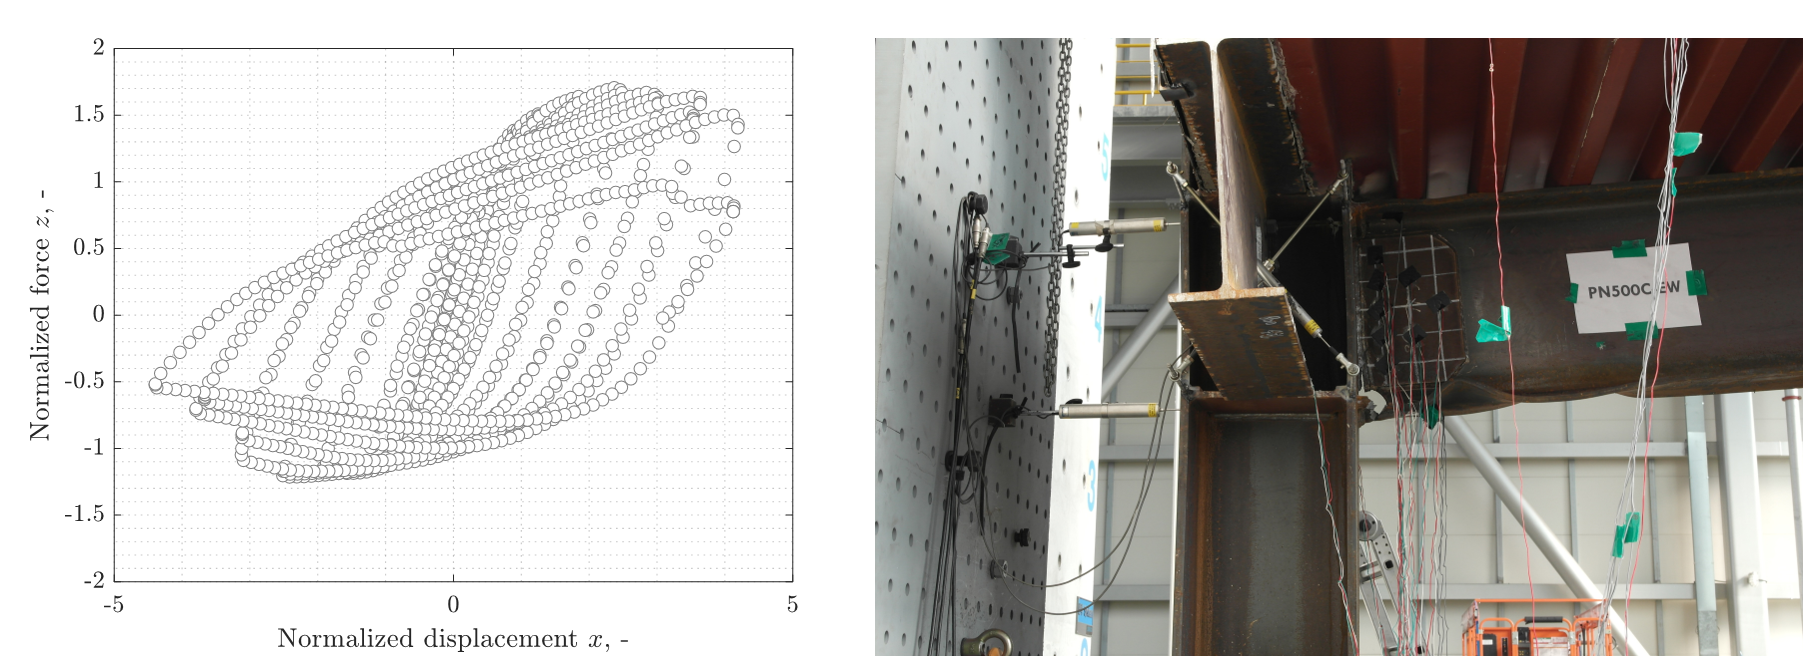
\includegraphics[height=.4\textheight]{testResult}
	\caption{Composite beam-column connections}
\end{figure}
\end{frame}

\begin{frame}{Example 3: Training Results}
\begin{figure}
	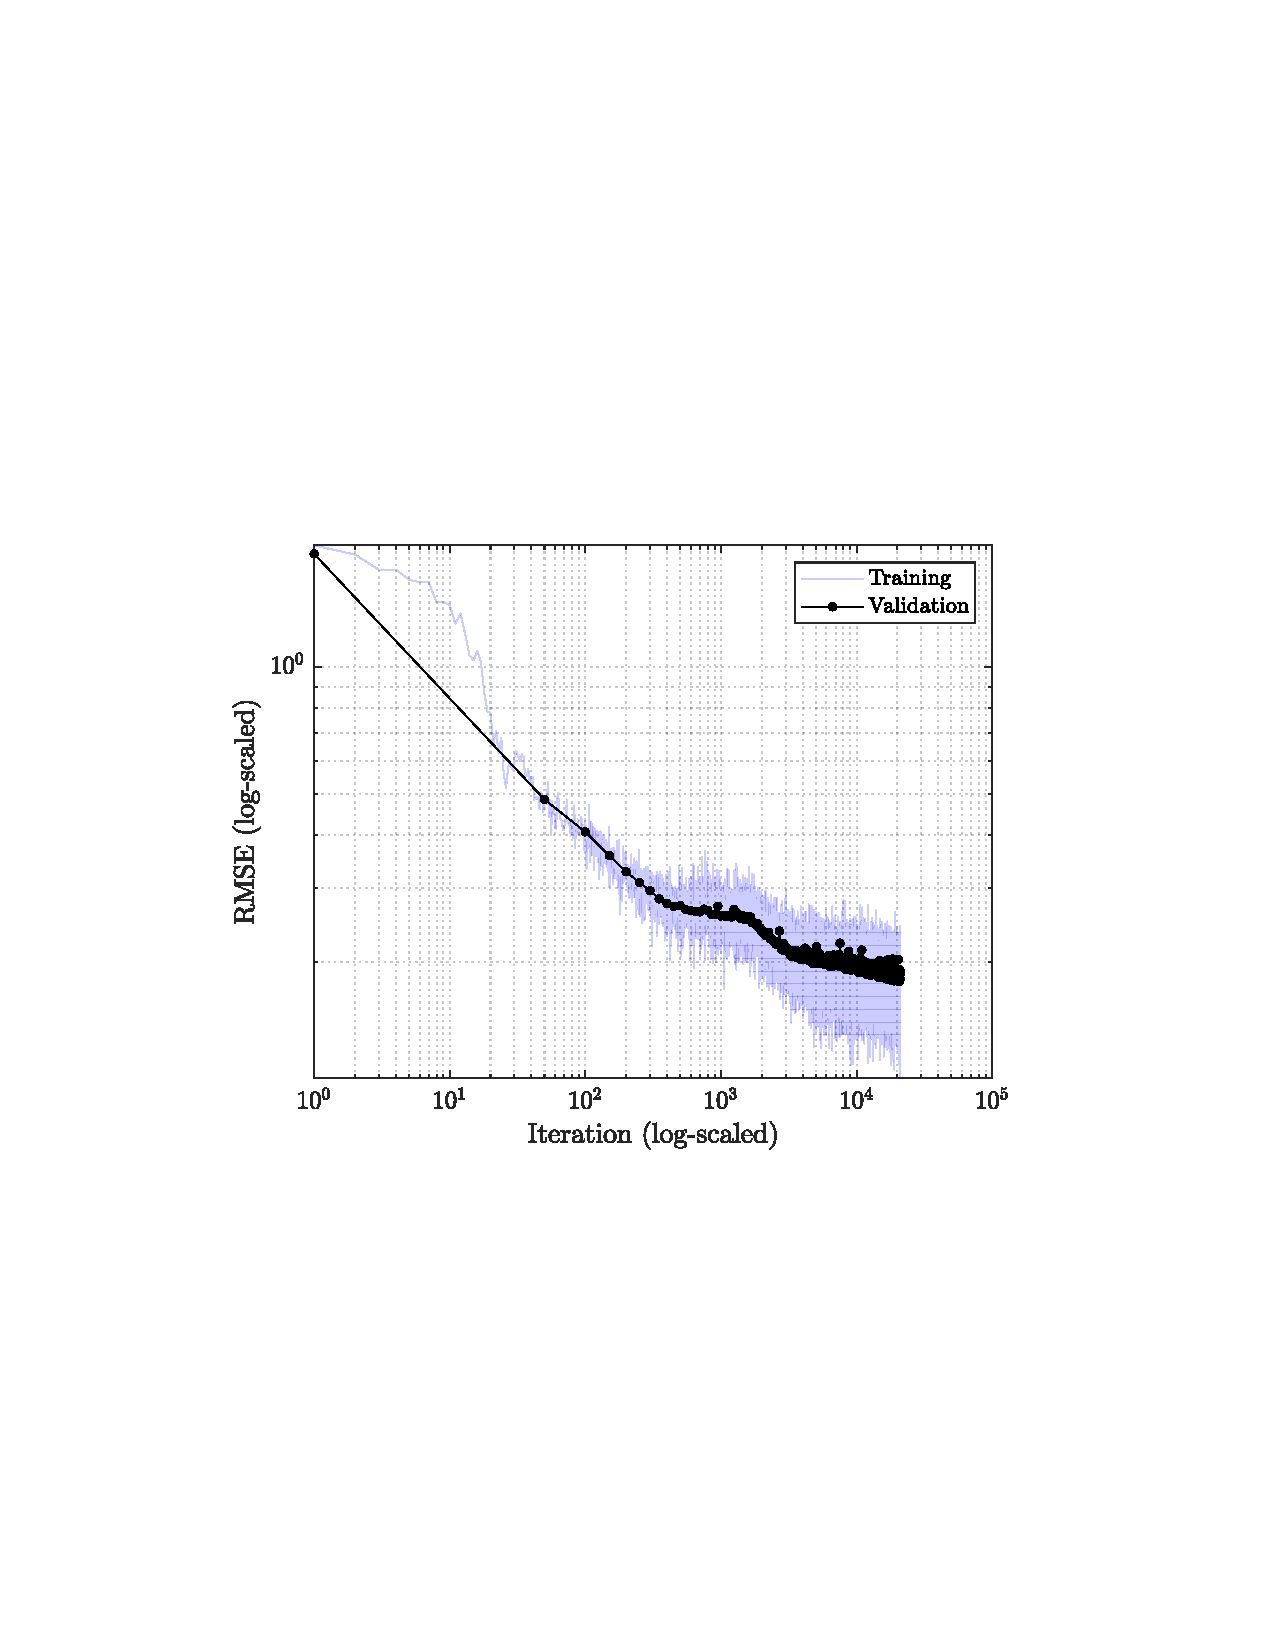
\includegraphics[height=.8\textheight]{neuralNetHysteresis03RMSE}
	\caption{Training history for Example 3}
\end{figure}
\end{frame}

\begin{frame}{Example 3: Validation Results}
\begin{figure}
	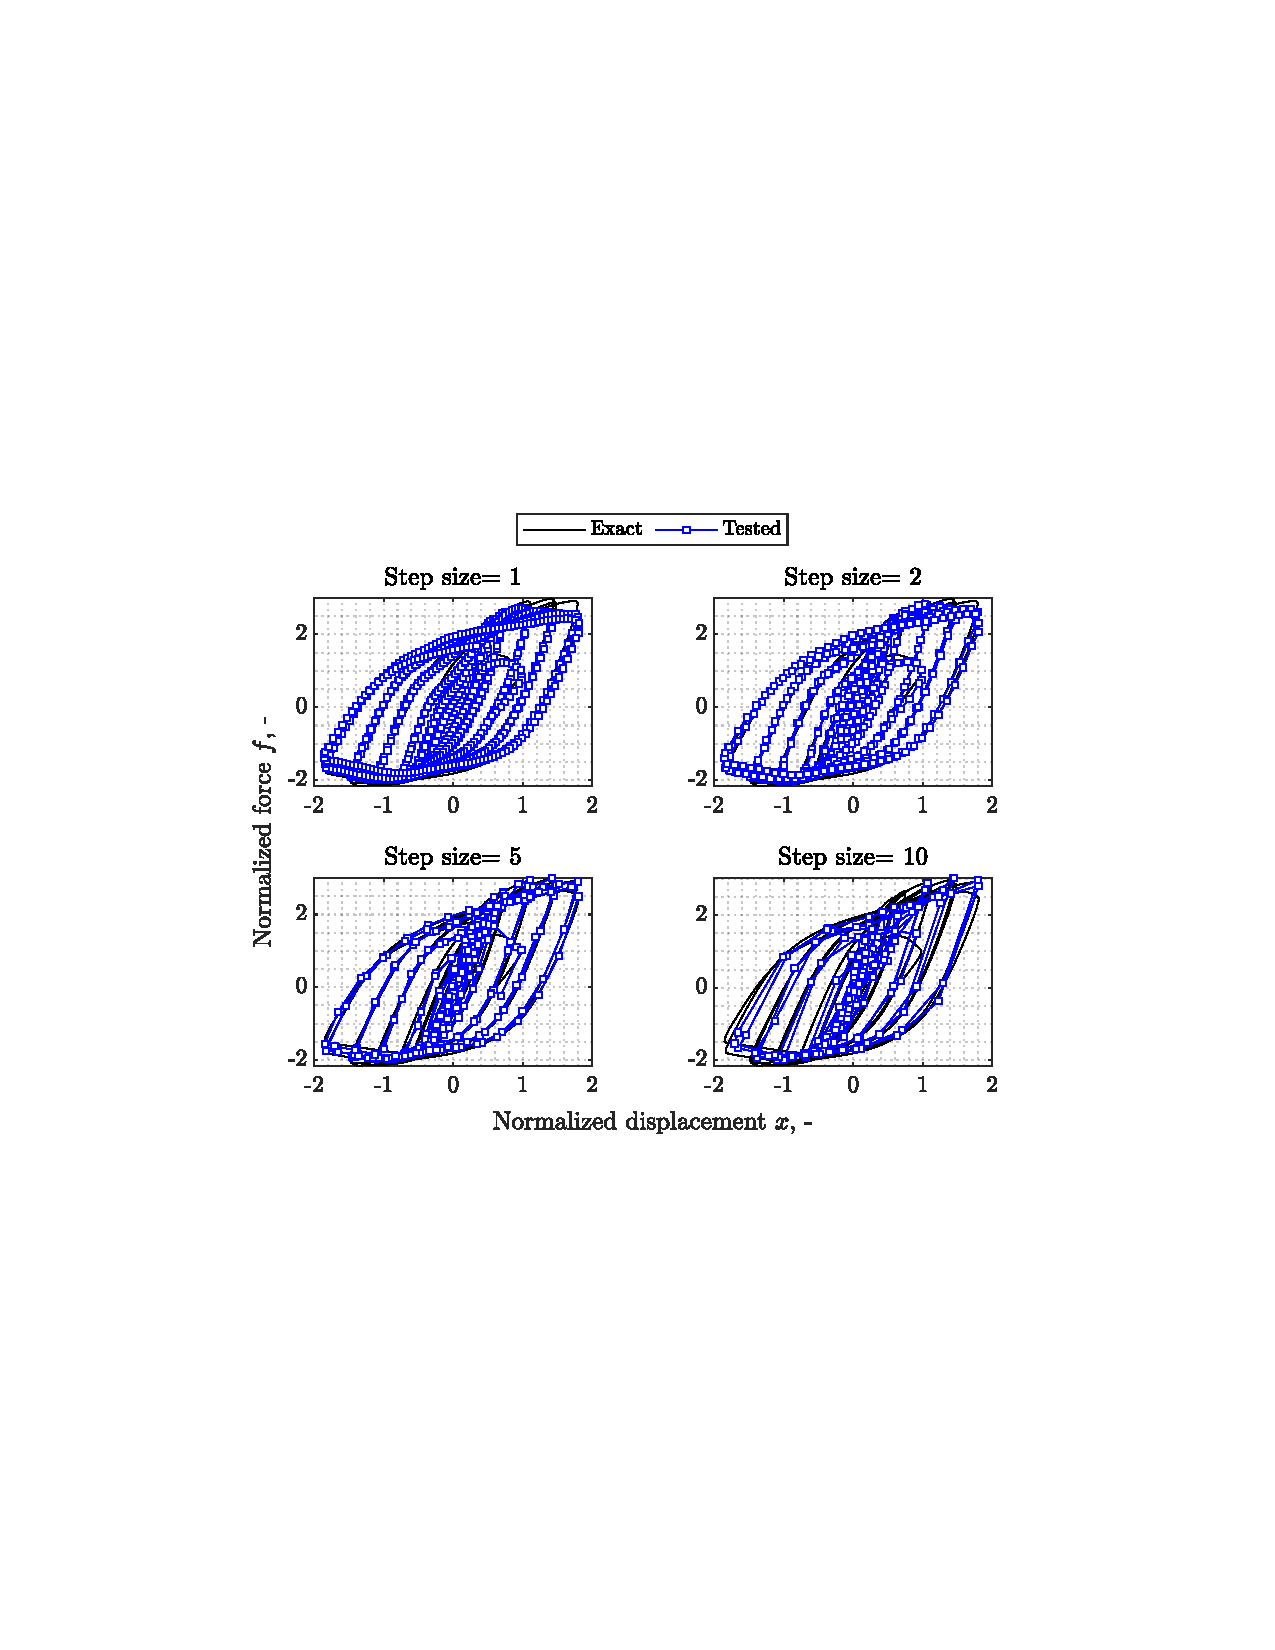
\includegraphics[height=.8\textheight]{neuralNetHysteresis03Test}
	\caption{Validation results}
\end{figure}
\end{frame}

\section{Summary and Conclusions}
\begin{frame}{Summary and Conclusions}
This study intends to provide a methodology for developing a neural network-based hysteresis model applicable to dynamic analysis using pseudo-static experiments. To this purpose, the authors devised a technique to incorporate into the learning set not only the input of pseudo-static trial outcomes, but also the input of large steps, such as 2, 5 and 10, etc. 

\begin{itemize}
	\item The predicted hysteresis loops agree well with the tested hysteresis loops considered step sizes for both datasets.
	\item  The model proposed in this study is an estimator that directly estimates the next step without an integration process.
\end{itemize}
\end{frame}

\begin{frame}
\small
\begin{itemize}
	\item SEEBUS 2020 (Canceled due to COVID-19) $\rightarrow$ First daughter (Saeun)
	\item SEEBUS 2022 (Japan) $\rightarrow$ Second daughter (Saeah)
	\item SEEBUS 2023 (Taiwan) $\rightarrow$ ? (Wishing Every SEEBUS Family A Happy And Blessed New Year)
\begin{figure}
	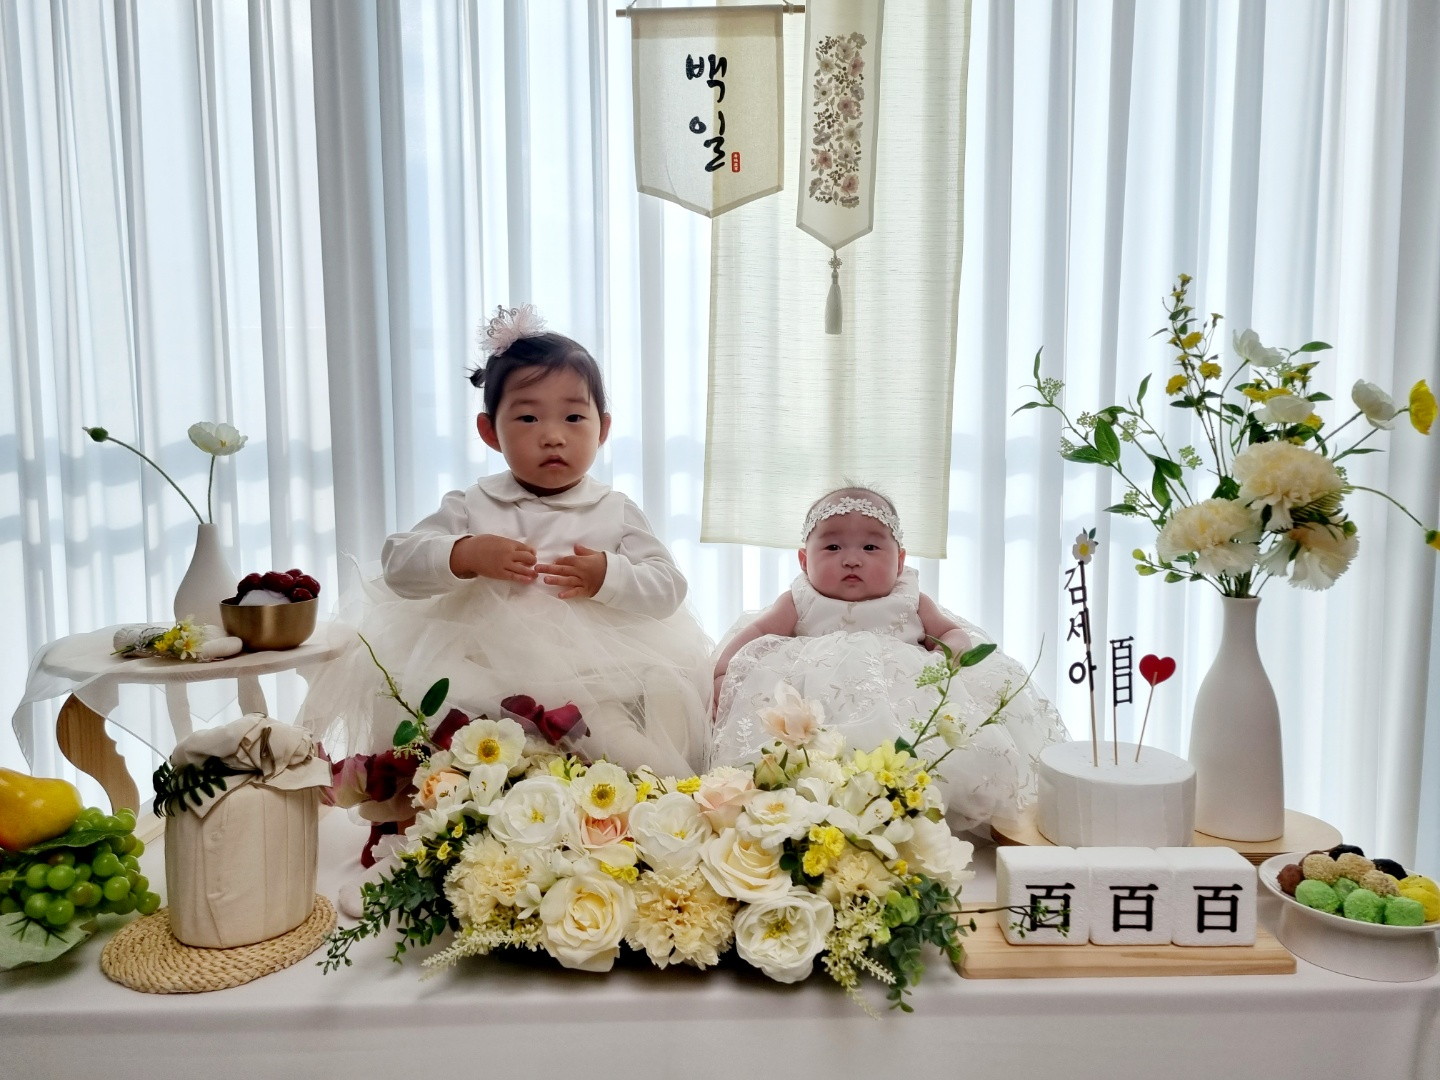
\includegraphics[height=.7\textheight]{KakaoTalk_20221203_210329893}
\end{figure}
\end{itemize}
\end{frame}
\endgroup
\end{document}

%\begin{frame}[fragile]
%\begin{itemize}
%	\item 사용프로그램: MATLAB\texttrademark R2019b for academic use
%	\item 적용 APP: Deep learning toolbox
%	\item 코드: 네트워크 구성 및 학습만 수록; 전/후처리는 생략
%\end{itemize}
%\scriptsize
%	\begin{lstlisting}{Matlab}
%numChannels = size(seq,1);
%numObservations = length(seq);
%
%idxTrain = 1:floor(0.5*numObservations);
%idxTest = floor(0.5*numObservations)+1:numObservations;
%dataTrain = seq(:, idxTrain);
%dataTest = seq(:, idxTest);
%
%XTrain = dataTrain(:, 1 : end - 1);
%TTrain = dataTrain(:, 2 : end);
%
%layers = [
%    sequenceInputLayer(numChannels)
%    lstmLayer(128)
%    fullyConnectedLayer(numChannels)
%    regressionLayer];
%
%options = trainingOptions('adam', ...
%    'MaxEpochs', 200, ...
%    'SequencePaddingDirection', 'left', ...
%    'Shuffle', 'every-epoch', ...
%    'Plots', 'training-progress', ...
%    'Verbose', 0);
%
%net = trainNetwork(XTrain,TTrain,layers,options);
%	\end{lstlisting}
%\end{frame}
%
%\begin{frame}{Training Progress}
%	\begin{figure}
%		\includegraphics[height=.45\textheight]{01_LSTMProgress}
%	\end{figure}
%	\begin{itemize}
%		\item 최대 200 epochs에 대해 학습: T01-T04의 네 수열에 대해 약 30분 간의 학습시간이 소요됨(CPU: Intel(R) Core(TM) i7-8550U CPU @ 1.80GHz   1.99 GHz, RAM 16.0GB의 통상적 사무용 노트북)
%		\item 전반적으로 높은 학습능률을 보였으며(RMSE/LOSS), 40 epochs 이후부터 유사한 성능을 가지는 모형들 사이에서 학습이 진행됨
%		\item 결과로 도시하진 않았으나 100 epochs에서 학습을 마친 모형의 경우 급작스런 변동을 충분히 예측하지 못하고, 2-3시간 가량의 데이터 지연 발생
%	\end{itemize}
%\end{frame}

